\begin{dang}{Câu hỏi lý thuyết về phản ứng oxi hóa khử}\end{dang}
\Noibat[\maunhan][][\faBookmark][]{Ví dụ mẫu}
%%%=============VD_1=============%%%
\begin{vd}[Nhận biết các quá trình vai trò của các chất]
	[][]Một nguyên tử nhôm (Al) chuyển thành ion $Al^{3+}$ thực hiện :
	\choice
	{%
		nhận thêm 3 electron (quá trình oxi hóa)
	}{%
		nhường đi 3 electron (quá trình khử)
	}{%
		nhận thêm 3 electron (quá trình khử)
	}{%
		\True nhường đi 3 electron (quá trình oxi hóa)
	}
	\loigiai{Quá trình oxi hóa  một chất là làm cho nguyên tử trong chất đó nhường electron hay làm tăng số oxi hóa của nguyên tử trong chất đó.\\
		Quá trình khử  một chất là làm cho nguyên tử trong chất đó nhận electron hay làm giảm số oxi hóa của nguyên tử trong chất đó.\\
		Ta thấy số oxi hóa của nhôm tăng (quá trình oxi hóa) \\
		$
		\begin{matrix}
			\overset{0}{Al}& \xrightarrow &\overset{+3}{Al} & + & 3e
		\end{matrix}
		$
	}
\end{vd}
%%%=============VD_2=============%%%
\begin{vd}[Nhận biết các quá trình vai trò của các chất]
	[][]Trong phản ứng : $Cl_2$+ $2KBr$$\xrightarrow$$Br_2$+$2KCl$, $Cl_2$ đóng vai trò
	\choice{%
		\True là chất oxi hóa
	}{%
		là chất khử
	}{%
		không bị oxi hóa, không bị khử
	}{%
		vừa bị oxi hóa, vừa bị khử.
	}
	\loigiai{Chất oxi hóa là chất nhận electron hay là chất có số oxi hóa giảm sau phản ứng.\\
		Chất khử là chất nhường electron hay là chất có số oxi hóa tăng sau phản ứng.\\
		Ta thấy số oxi hóa của Cl giảm :\\
		$
		\begin{matrix}
			Cl_2 & + & 2e & \xrightarrow & 2Cl^{-}
		\end{matrix}
		$
	}
\end{vd}
%

%%%=============VD_3=============%%%
\begin{vd}[Nhận biết phản ứng oxi hóa khử]
	[][]
	Phản ứng nào sau đây \indam[black]{không phải} phản ứng oxi hóa khử
	\choice{
		$2NaOH$ + $Cl_2$ $\xrightarrow$ $NaCl$ + $NaClO$ + $H_2O$
	}{
		\True $CaCO_3$ $\xrightarrow[$t^\circ$]$ $CaO$ + $CO_2$
	}{
		$2KClO_3$ $\xrightarrow[$t^\circ$]$ $2KCl$ + $3O_2$
	}{
		$Fe$+ $2HCl$ $\xrightarrow$ $FeCl_2$ + $H_2$
	}
	\loigiai{%
		Phản ứng oxi hóa - khử là phản ứng  hóa học trong đó có sự thay đổi số oxi hóa.\\
		Phản ứng không phải là phản ứng oxi hóa - khử là phản ứng không có sự thay đổi số oxi hóa của các nguyên tố\\
		Ta có:\\
		$
		\begin{matrix}
			2NaOH  & + & \overset{0}{Cl}_{2} & \xrightarrow & \overset{\vphantom{+1}}{Na}\overset{-1}{Cl} & + & \overset{\vphantom{+1}}{Na}\overset{+1}{Cl}O  & + & H_2O\\
		\end{matrix}
		$\\
		$
		\begin{matrix}
			\overset{\vphantom{+4}}{Ca}\overset{+4}{C}\overset{\vphantom{-2}}{O_3} & \xrightarrow& \overset{+2}{Ca}O & + & \overset{+4}{C}\overset{\vphantom{+4}}{O_2}\\
		\end{matrix}
		$\\
		$
		\begin{matrix}
			\overset{\vphantom{-2}}{2K}\overset{+5}{Cl}\overset{\vphantom{-2}}{O_3} & \xrightarrow& \overset{\vphantom{-2}}{2K}\overset{-1}{Cl} & + & 3\!{\overset{\scriptsize-2}{O}}\!_2\\
		\end{matrix}
		$\\
		$
		\begin{matrix}
			\overset{0}{Fe}& + & 2\overset{+1}{H}Cl & \xrightarrow & \overset{+2}{Fe}\overset{\vphantom{-2}}{Cl_2} & + & {\overset{0}{H}}_2 \\
		\end{matrix}
		$\\
		\indam{Nhận xét: }Phản ứng B không có sự thay đổi số oxi hóa của các nguyên tố. $\Rightarrow$ Phản ứng B không phải là phản ứng oxi hóa - khử
	}
\end{vd}
%
%

%%%=============VD_4=============%%%
\begin{vd}[Nhận biết phản ứng oxi hóa khử]
	[][]Cho các phản ứng sau đây:
	\begin{enumerate}[a)]
		\item $C + O_{2} \xrightarrow[$t^\circ$] CO_{2}$
		\item $CaO +  H_{2}O \xrightarrow Ca(OH)_{2}$
		\item $CuO + H_{2} \xrightarrow[$t^\circ$] Cu + O_2$
		\item $2KMnO_4 \xrightarrow[$t^\circ$] K_2MnO_4 + MnO_2 + H_2O$
		\item $Cl_2 + 2KOH \xrightarrow KCl + KClO + H_2O$
		\item $Fe_3O_4 + 8HCl \xrightarrow 2FeCl_3 + FeCl_2 + 4H_2O$
	\end{enumerate}
	Số phản ứng thuộc loại phản ứng oxi hóa - khử là:
	\choice{2}{\True 4}{3}{5}
	\loigiai{%
		Phản ứng oxi hóa khử là phản ứng hóa học trong đó có sự thay đổi số oxi hóa của một số nguyên tố.
		\begin{enumerate}[a)]
			\item $\overset{0}{C} + \overset{0}{O}_{2} \xrightarrow[$t^\circ$] \overset{+4}{C}\overset{-2}{O}_{2}$
			\item $\overset{+2}{Ca}\overset{-2}{O} +  \overset{+1}{H_{2}}\overset{-2}{O} \xrightarrow \overset{+2}{Ca}(\overset{-2}{O}\overset{+1}{H})_{2}$
			\item $\overset{+2}{Cu}\overset{-2}{O} + \overset{-2}{H}_{2} \xrightarrow[$t^\circ$] \overset{0}{Cu} + \overset{+1}{H}_2\overset{-2}{O}$
			\item $2K\overset{+7}{Mn}\overset{-2}{O}_4 \xrightarrow[$t^\circ$] K_2\overset{+6}{Mn}O_4 + \overset{0}{O}_2 + \overset{+6}{Mn}O_{2}$
			\item $\overset{0}{Cl}_2 + 2KOH \xrightarrow K\overset{-1}{Cl} + K\overset{+1}{Cl}O + H_2O$
			\item $\overset{+8/3}{Fe_3}\overset{-2}{O_4} + 8\overset{+1}{H}\overset{-1}{Cl} \xrightarrow 2\overset{+3}{Fe}Cl_3 + \overset{+2}{Fe}\overset{-1}{Cl}_2 + 4\overset{+1}{H}_2O$
		\end{enumerate}
		\indam{Nhận xét:} Phản ứng a), c), d), e) có sự thay đổi số oxi hóa của các nguyên tố. $\Rightarrow$ Phản ứng a), c), d), e) là phản ứng oxi hóa - khử
	}
\end{vd}
%%%=============VD_5=============%%%
\begin{vd}[Cân bằng phản ứng oxi hóa khử]
	[][]Lập phương trình phản ứng oxi hóa - khử sau đây:
	$MnO_2$ + $HCl$ $\xrightarrow$ $MnCl_2$ + $Cl_2$ + $H_2O$
	\loigiai{
		\begin{cacbuoc}
			\item Xác định số oxi hóa của các nguyên tố :\\
			$\overset{+4}{Mn}O_2 + H\overset{-1}{Cl} \xrightarrow \overset{+2}{Mn}Cl_2 + \overset{0}{Cl_2} + H_2O$
			\item Quá trình cho - nhận electron\\
			$
			\begin{matrix}
				2\overset{-1}{Cl} & \xrightarrow& Cl_2 & + & 2e\\
				\overset{+4}{Mn} &  + & 2e & \xrightarrow & \overset{+2}{Mn}
			\end{matrix}
			$
			\item Đặt hệ số \\
			$
			\begin{matrix}
				1x|~2\overset{-1}{Cl} & \xrightarrow& Cl_2 & + & 2e\\
				1x|~\overset{+4}{Mn} &  + & 2e & \xrightarrow & \overset{+2}{Mn}
			\end{matrix}
			$
			\item Phương trình hóa học
			\boxct{$MnO_2 + 4HCl \xrightarrow MnCl_2 + Cl_2 + 2H_2O$}
		\end{cacbuoc}
	}
\end{vd}
%%%=============VD_6=============%%%
\begin{vd}[Cân bằng phản ứng oxi hóa - khử]
	[][Nguồn:CĐA 2010] Cho phản ứng:
	$\mathrm{Na}_2 SO_3+\mathrm{KMnO}_4+\mathrm{NaHSO}_4$ $\xrightarrow$ $\mathrm{Na}_2 SO_4+\mathrm{MnSO}_4+K_2 SO_4+H_2 O$.Tổng hệ số của các chất (là những số nguyên, tối giản) trong phương trình phản ứng là
	\choice
	{23}
	{27}
	{47}
	{31}
	\loigiai{
		\begin{cacbuoc}
			\item Xác định số oxi hóa của các nguyên tố :\\
			$Na_2\overset{+4}{S}O_3$ + $K\overset{+7}{Mn}O_4$ + $NaHSO_4$ $\xrightarrow$ $Na_2\overset{+6}{S}O_4$ + $\overset{+2}{Mn}SO_4$ + $K_2SO_4$ + $H_2 O$
			\item Quá trình cho - nhận electron\\
			$
			\begin{matrix}
				\overset{+7}{Mn} &  + & 5e & \xrightarrow & \overset{+2}{Mn}\\
				\overset{+4}{S} & \xrightarrow& \overset{+6}{Mn} & + & 2e
			\end{matrix}
			$
			\item Đặt hệ số \\
			$
			\begin{array}{lllll}
				2x|~\overset{+7}{Mn} &  + & 5e & \xrightarrow & \overset{+2}{Mn}\\
				5x|~\overset{+4}{S} & \xrightarrow& \overset{+6}{Mn} & + & 2e
			\end{array}
			$\\
			\item Phương trình hóa học\\
			Hệ số 5 điền cho S ($5Na_2SO_3$ và $?Na_2SO_4$). Hệ số 2 điền cho Mn ($2KMnO4$ và $2MnO4$).
			
			\GSND[][\faComment]{Phân tích:}Hệ số của $\mathrm{Na}_2 \mathrm{SO}_3, \mathrm{KMnO}_4, \mathrm{MnSO}_4$ và $\mathrm{K}_2 \mathrm{SO}_4$ đã được xác định.\\
			Do gốc $\mathrm{SO}_4^{2-}$ là sản phẩm oxi hóa của $\mathrm{SO}_3^{2-}$ đồng thời cũng là sản phẩm của chất làm nhiệm vụ môi trường $\mathrm{NaHSO}_4$. Do vậy cần tìm hệ số của $\mathrm{Na}_2 \mathrm{SO}_4, \mathrm{NaHSO}_4$ và $\mathrm{H}_2 \mathrm{O}$ bằng phương pháp bảo toàn nguyên tố.
			%
			\noindent Đặt $x$ là hệ số của $\mathrm{Na}_2 \mathrm{SO}_4$ và $ y$ là hệ số của $\mathrm{H_2O}$ .\\
			- Bảo toàn số nguyên tử  $H\Rightarrow$ hệ số của $NaHSO_4$ là $2y$\\
			$5\mathrm{Na}_2 SO_3+2\mathrm{KMnO}_4+2y\mathrm{NaHSO}_4$ $\xrightarrow$ $x\mathrm{Na}_2 SO_4+2\mathrm{MnSO}_4+K_2 SO_4+yH_2 O$\\
			- Bảo toàn số nguyên tử $S \Rightarrow(5+2 y)=(x+2+1) \Rightarrow(x-2 y)=2$ (*)\\
			- Bảo toàn số nguyên tử $O$
			$\Rightarrow(15+8+8 y)=(4 x+12+y) \Rightarrow(4 x-7 y)=11$(**)\\
			Từ (*) và (**) $\Rightarrow x=8 ; y=3$
			\boxct[\mauphu]{$5\mathrm{Na}_2 SO_3+2\mathrm{KMnO}_4+6\mathrm{NaHSO}_4$ $\xrightarrow$ $8\mathrm{Na}_2SO_4+2\mathrm{MnSO}_4+K_2 SO_4+3H_2 O$}
		\end{cacbuoc}
	}
\end{vd}
%%%=============VD_7=============%%%
\begin{vd}[Cân bằng phản ứng oxi hóa - khử]
	Cân bằng các phản ứng oxi hóa khử sau bằng phương pháp \indam[black]{thăng bằng electron}:
	\begin{enumerate}
		\item $\mathrm{KMnO}_4+\mathrm{HCl}$ $\xrightarrow$ $\mathrm{MnCl}_2+\mathrm{Cl}_2+\mathrm{KCl}+H_2O$
		\item $K_2\mathrm{Cr}_2O_7+\mathrm{HCl} $ $\xrightarrow$ $ \mathrm{CrCl}_3+\mathrm{Cl}_2+\mathrm{KCl}+H_2O$
	\end{enumerate}
	\loigiai{
		\begin{enumerate}[(1)]
			\item $\mathrm{KMnO}_4+\mathrm{HCl} $ $\xrightarrow$ $ \mathrm{MnCl}_2+\mathrm{Cl}_2+\mathrm{KCl}+H_2O$
			\begin{cacbuoc}
				\item Xác định số oxi hóa của các nguyên tố :\\
				$K\overset{+7}{Mn}O_4 + H\overset{-1}{Cl} \xrightarrow \overset{+2}{Mn}Cl_2 + \overset{0}{Cl_2} + H_2O$
				\item Quá trình cho - nhận electron\\
				$
				\begin{matrix}
					2\overset{-1}{Cl} & \xrightarrow& Cl_2 & + & 2e\\
					\overset{+7}{Mn} &  + & 5e & \xrightarrow & \overset{+2}{Mn}
				\end{matrix}
				$
				\item Đặt hệ số \\
				$
				\begin{array}{lccccc}
					5x\biggl|&2\overset{-1}{Cl} & \xrightarrow& Cl_2 & + & 2e\\
					2x\biggl|&\overset{+7}{Mn} &  + & 5e & \xrightarrow & \overset{+2}{Mn}
				\end{array}
				$
				\item Phương trình hóa học\\
				Đặt hệ số 2 cho Mn ($2MnCl_2$ và $2KMnO_4$).Đặt hệ số 5 cho Cl ($5Cl_2$ và $?HCl$)\\
				- Bảo toàn K: $\Rightarrow 2KCl $\\
				$\Rightarrow 2\mathrm{KMnO}_4+?\mathrm{HCl} $ $\xrightarrow$ $ 2\mathrm{MnCl}_2+ 5\mathrm{Cl}_2+2\mathrm{KCl}+H_2O$
				\GSND[][\faComment]{Phân tích:}HCl tham gia vào quá trình oxi hóa (tạo ra $5Cl_2$)  và làm môi trường tạo muối ($2MnCl_2$ và $2KCl$ ).Như vậy bảo toàn Cl $\Rightarrow 16HCl $ và bảo toàn H $\Rightarrow 8H_2O $
				\boxct{$2\mathrm{KMnO}_4+16\mathrm{HCl} $ $\xrightarrow$ $ 2\mathrm{MnCl}_2+5\mathrm{Cl}_2+2\mathrm{KCl}+8H_2O$}
			\end{cacbuoc}
			\item $K_2\mathrm{Cr}_2O_7+\mathrm{HCl} $ $\xrightarrow$ $ \mathrm{CrCl}_3+\mathrm{Cl}_2+\mathrm{KCl}+H_2O$
			\begin{cacbuoc}
				\item Xác định số oxi hóa của các nguyên tố :\\
				$K_2\mathrm{\overset{+6}{Cr}}_2O_7+\mathrm{H\overset{-1}{Cl}} $ $\xrightarrow$ $ \mathrm{\overset{+3}{Cr}Cl}_3+\overset{0}{Cl}_2+\mathrm{KCl}+H_2O$
				\item Quá trình cho - nhận electron\\
				$
				\begin{matrix}
					2\overset{+6}{Cr} &  + & 6e & \xrightarrow & 2\overset{+3}{Cr}\\
					2\overset{-1}{Cl} & \xrightarrow& Cl_2 & + & 2e\\
				\end{matrix}
				$
				\item Đặt hệ số \\
				$
				\begin{array}{lccccc}
					1x\biggl|&2\overset{+6}{Cr} &  + & 6e & \xrightarrow & 2\overset{+3}{Cr}\\
					3x\biggl|&2\overset{-1}{Cl} & \xrightarrow & Cl_2 & + & 2e\\
				\end{array}
				$
				\item Phương trình hóa học\\
				Đặt hệ số  cho Cr ( $K_2Cr_2O_7$ và $2CrCl_3$).Đặt hệ số 3 cho Cl ( $3Cl_2$ và $?HCl$).\\
				- Bảo toàn K: $\Rightarrow 2KCl $\\
				$K_2\mathrm{Cr}_2O_7+?\mathrm{HCl} $ $\xrightarrow$ $ 2\mathrm{CrCl}_3+3\mathrm{Cl}_2+2\mathrm{KCl}+H_2O$
				\GSND[][\faComment]{Phân tích:}HCl tham gia vào quá trình oxi hóa (tạo ra $3Cl_2$)  và làm môi trường tạo muối ($2CrCl_3$ và $2KCl$ ).Như vậy bảo toàn Cl $\Rightarrow 14HCl $ và bảo toàn H $\Rightarrow 7H_2O $
				\boxct{$K_2\mathrm{Cr}_2O_7+14\mathrm{HCl} $ $\xrightarrow$ $ 2\mathrm{CrCl}_3+3\mathrm{Cl}_2+2\mathrm{KCl}+7H_2O$}
			\end{cacbuoc}
		\end{enumerate}
	}
\end{vd}
%%%=============VD_8=============%%%
\begin{vd}[Cân bằng phản ứng oxi hóa - khử]
	Cân bằng các phản ứng oxi hóa khử sau bằng phương pháp thăng bằng electron:
	\begin{enumerate}[(a)]
		\item $\mathrm{FeS}_2+O_2$ $\xrightarrow$ $\mathrm{Fe}_2O_3+SO_2$
		\item $P+NH_4\mathrm{HClO}_4$ $\xrightarrow$ $H_3PO_4+\mathrm{Cl}_2+N_2+H_2O$
	\end{enumerate}
	\loigiai{
		\begin{enumerate}[(a)]
			\item $\mathrm{FeS}_2+O_2$ $\xrightarrow$ $\mathrm{Fe}_2O_3+SO_2$
			\begin{cacbuoc}
				\item Xác định số oxi hóa của các nguyên tố :\\
				$\mathrm{\overset{+2}{Fe}\overset{-1}{S}}_2+\overset{0}{O}_2$ $\xrightarrow$ $ \mathrm{\overset{+3}{Fe}}_2\overset{-2}{O}_3+\overset{+4}{S}\overset{-2}{O}_2$
				\item Quá trình cho - nhận electron\\
				$
				\begin{array}{ccccccc}
					\left(\mathrm{FeS}_2\right)^0 &   \xrightarrow & \mathrm{Fe}^{+3} & + & 2 \mathrm{~S}^{+4}& + &11\mathrm{e} \\
					\mathrm{O}_2 & + & 4\mathrm{e} &   \xrightarrow & 2\mathrm{O}^{-2}& & \\
				\end{array}
				$
				\item Đặt hệ số \\
				$
				\begin{array}{rccccccc}
					4x\biggl|&\left(\mathrm{FeS}_2\right)^0 &   \xrightarrow & \mathrm{Fe}^{+3} & + & 2 \mathrm{~S}^{+4}& + &11\mathrm{e} \\
					11x\biggl|& \mathrm{O}_2 & + & 4\mathrm{e} &   \xrightarrow & 2\mathrm{O}^{-2}& & \\
				\end{array}
				$
				\item Phương trình hóa học\\
				Đặt hệ số 4 cho Fe ( $4FeS_2$ và $2Fe_2O_3$).Đặt hệ số 11 cho O ($11O_2$).\\
				- Bảo toàn S: $\Rightarrow 8SO_2 $.Kiểm tra O hai vế
				\boxct{$4\mathrm{FeS}_2+11O_2$ $\xrightarrow[$t^\circ$]$ $ 2\mathrm{Fe}_2O_3+8SO_2$}
			\end{cacbuoc}
			\item $P+NH_4\mathrm{ClO}_4$ $\xrightarrow$ $ H_3PO_4+\mathrm{Cl}_2+N_2+H_2O$
			\begin{cacbuoc}
				\item Xác định số oxi hóa của các nguyên tố :\\
				$\overset{0}{P}+\overset{-3}{N}H_4\mathrm{\overset{+7}{Cl}O}_4$ $\xrightarrow$ $ H_3\overset{+5}{P}O_4+\mathrm{\overset{0}{Cl}}_2+\overset{0}{N}_2+H_2O$
				\item Quá trình cho - nhận electron\\
				$
				\begin{array}{ccccccccc}
					\overset{0}{P}& \xrightarrow  &\overset{+5}{P}& + & 5e&&&&\\
					2\overset{-3}{N}&+ &2\overset{+7}{Cl}&+ & 8e & \xrightarrow  &\overset{0}{Cl}_2& + & \overset{0}{N}_2\\
				\end{array}
				$
				\item Đặt hệ số \\
				$
				\begin{array}{rccccccccc}
					8x\bigg|&\overset{0}{P}& \xrightarrow  &\overset{+5}{P}& + & 5e&&&&\\
					5x\bigg|&2\overset{-3}{N}&+ &2\overset{+7}{Cl}&+ & 8e & \xrightarrow  &\overset{0}{Cl}_2& + & \overset{0}{N}_2\\
				\end{array}
				$
				\item Phương trình hóa học\\
				Đặt hệ số 8 cho P ( $8P$ và $8H_3PO_4$).Đặt hệ số 5 cho Cl và N ($10NH4ClO_4$, $5Cl_2$ và $5N_2$).\\
				- Bảo toàn H: $\Rightarrow 8H_2O $.Kiểm tra O hai vế
				\boxct{$8P+10NH_4\mathrm{ClO}_4$ $\xrightarrow$ $ 8H_3PO_4+5\mathrm{Cl}_2+5\mathrm{N}_2+8H_2O$}
			\end{cacbuoc}
		\end{enumerate}
	}
\end{vd}
%%%=============VD_9=============%%%
\begin{vd}[Cân bằng phản ứng oxi hóa - khử]
	Cân bằng phản ứng hóa học sau theo phương pháp thăng bằng electron.
	$\mathrm{FeO}+HNO_3 $ $\xrightarrow$ $ \mathrm{Fe}\left(NO_3\right)_3+ NO_2 + NO + H_2 O \quad\left(n_{NO_2}: n_{NO}=a: b\right)$
	\loigiai{
		\begin{cacbuoc}
			\item Xác định số oxi hóa của các nguyên tố :\\
			$\mathrm{\overset{+2}{Fe}O}+H\overset{+5}{N}O_3 $ $\xrightarrow$ $ \mathrm{\overset{+3}{Fe}}\left(NO_3\right)_3+ \overset{+4}{N}O_2 + \overset{+2}{N}O + H_2 O$
			\item Quá trình cho - nhận electron, đặt chéo hệ số\\
			\begin{tabular}{r|cccccccc}
				&$\overset{+5}{N}$&+&1e & $\xrightarrow$ & $\overset{+4}{N}$&$\big|x\;a$&&\\
				&$\overset{+5}{N}$&+&3e &$\xrightarrow$& $\overset{+2}{N}$&$\big|x\; b$&&\\
				\cline{2-8}
				&$(a+b)\overset{+5}{N}$&+&$(a+3b)e$&  $\xrightarrow$ &$aNO_2$&+&$bNO$&\\
				&$\overset{+2}{Fe}$& $\xrightarrow$ &$\overset{+3}{Fe}$ & + & 1e& & &\\
				\hline
				\indam{1X}&$(a+b)\overset{+5}{N}$&+&$(a+3b)e$&  $\xrightarrow$ &$aNO_2$&+&$bNO$&\\
				\indam{(a+3b)X}&$\overset{+2}{Fe}$ &  $\xrightarrow$  & $\overset{+3}{Fe}$& + & $1\mathrm{e}$&&&\\
			\end{tabular}
			\item Phương trình hóa học\\
			Đặt hệ số 1 cho N( $aNO_2$ và $bNO$). Đặt hệ số (a+3b) cho Fe $\big((a+3b)FeO \;\text{và} \;(a+3b)Fe{(NO_3)}_{3} \big)$\\
			- Bảo toàn N: $\Rightarrow (4a+10b)HNO_3 $. Bảo toàn H $\Rightarrow (2a+5b)H_2O $. Kiểm tra O hai vế
			\boxct{$(a+3b)\mathrm{FeO}+(4a+10b)HNO_3$ $\xrightarrow$ $ (a+3b)\mathrm{Fe}\left(NO_3\right)_3+ aNO_2 + bNO +(2a+5b) H_2 O$}
		\end{cacbuoc}
	}
\end{vd}
%%%=============VD_10=============%%%
\begin{vd}[Cân bằng phản ứng oxi hóa - khử]
	Cân bằng phản ứng oxi khử sau đây bằng phương pháp thăng bằng electron: \\
	$\mathrm{Fe}_x O_y+HNO_3 $ $\xrightarrow$ $ \mathrm{Fe}\left(NO_3\right)_3+NO+H_2O$
	\loigiai{
		\begin{cacbuoc}
			\item Xác định số oxi hóa của các nguyên tố :\\
			$\mathrm{\overset{+2y/x}{Fe_x}} O_y+H\overset{+5}{N}O_3 $ $\xrightarrow$ $ \mathrm{\overset{+3}{Fe}}\left(NO_3\right)_3+\overset{+2}{N}O+H_2O$
			\item Quá trình cho - nhận electron, đặt chéo hệ số\\
			\begin{tabular}{r|ccccc}
				3X&$x\overset{+2y/x}{Fe}$& $\xrightarrow$ &$x\overset{+3}{Fe}$&+ &$(3x-2y)e$\\
				$(3x-2y)X$&$\overset{+5}{N}$&+&$3e$&$\xrightarrow$ &$\overset{+2}{N}$\\
			\end{tabular}
			\item Phương trình hóa học\\
			Đặt hệ số 3 cho Fe ($3xFe{(NO_3)}_3$ và $3Fe_xO_y$). Đặt hệ số (3x-2y) cho N $\big((3x-2y)NO \;\text{và} \;?HNO_3\big)$\\
			- Bảo toàn N: $\Rightarrow (12x-2y)HNO_3 $. Bảo toàn H $\Rightarrow (6x-y)H_2O $. Kiểm tra O hai vế
			\boxct{$3\mathrm{Fe}_x O_y+(12x-2y)HNO_3 $ $\xrightarrow$ $ 3x\mathrm{Fe}\left(NO_3\right)_3+(3x-2y)NO+(6x-y)H_2O$}
		\end{cacbuoc}
	}
\end{vd}
%%%%%=====================Bài tập tự luyện Dạng 1==========================%%%
\Noibat[\maunhan][][\faBook][]{Bài tập tự luyện}
%%%%============Phần trắc nghiệm============%%%
\phan{Bài tập tự luận}
%%%=============SOẠN BT===============%%%
\Opensolutionfile{ansbth}[Ans/LGBT-C04B01_Dang1]
\Opensolutionfile{ansbt}[Ans/AnsBT-C04B01_Dang1]
	%%%=============BT_1=============%%%
	\begin{bt}[Xác định số oxi hóa]
		Xác định số oxi hóa của mỗi nguyên tử nguyên tố trong các chất hoặc ion sau: $\mathrm{Al}_2O_3; \mathrm{CaF}_2$; $\mathrm{Fe}_2O_3; \mathrm{Na}_2CO_3; \mathrm{KAl}\left(SO_4\right)_2; NO_3^{-}; NH_4^{+}; \mathrm{MnO}_4^{-}$
	\end{bt}
	%%%=============BT_2=============%%%
	\begin{bt}[Xác định số oxi hóa]
		Xác định số oxi hóa của mỗi nguyên tử trong các phân tử và ion sau đây:
		\begin{enumerate}
			\item $H_2SO_3$;
			\item $\mathrm{Al}(OH)_4^{-}$;
			\item $\mathrm{NaAlH}_4$;
			\item $NO_2^{-}$.
		\end{enumerate}
	\end{bt}
	%%%=============BT_3=============%%%
	\begin{bt}[Xác định số oxi hóa]
		Tính số oxi hóa của nguyên tử đánh dấu * trong các chất và ion dưới đây:
		\begin{enumerate}
			\item $K_2\stackrel{*}{\mathrm{Cr}} O_7; \mathrm{KMnO}_4; \stackrel{*}{\mathrm{~K}} \stackrel{*}{\mathrm{ClO}} K_4; \stackrel{*}{\mathrm{~N}} H_4NO_3$
			\item $\stackrel{*}{\mathrm{~A}} O_2^{-}; \stackrel{*}{PO} O_4^{3-}; \stackrel{*}{C} \mathrm{ClO}_3^{-}; \stackrel{*}{SO_4^{2-}}$
		\end{enumerate}
	\end{bt}
	%%%=============BT_4=============%%%
	\begin{bt}[Xác định số oxi hóa]
		Xác định số oxi hóa của nguyên tử $\mathrm{Fe}$ và $S$ trong các chất sau:
		\begin{enumerate}
			\item $\mathrm{Fe}, \mathrm{FeO}, \mathrm{Fe}_2O_3, \mathrm{Fe}(OH)_3, \mathrm{Fe}_3O_4$.
			\item $S, H_2\mathrm{~S}, SO_2, SO_3, H_2SO_4, \mathrm{Na}_2SO_3$.
		\end{enumerate}
	\end{bt}
	%%%=============BT_5=============%%%
	\begin{bt}[Xác định số oxi hóa]
		Xác định số oxi hóa của các nguyên tố trong các chất và ion sau:
		\begin{enumerate}
			\item $\mathrm{Fe}, N_2, SO_3, H_2SO_4, \mathrm{CuS}, \mathrm{Cu}_2\mathrm{~S}, \mathrm{Na}_2O_2, H_3\mathrm{AsO}_4$.
			\item $\mathrm{Br}_2, O_3, \mathrm{HClO}_3, \mathrm{KClO}_4, \mathrm{NaClO}, NH_4NO_3, \mathrm{~N}_2O, \mathrm{NaNO}_2$.
		\end{enumerate}
	\end{bt}
	%%%=============BT_6=============%%%
	\begin{bt}[Xác định chất oxi hóa, chất khử và quá trình]
		Xác định chất oxi hóa, chất khử, quá trình oxi hóa, quá trình khử trong các phản ứng sau:
		\begin{enumerate}
			\item $\mathrm{Ag}^{+}+\mathrm{Fe}^{2+} $ $\xrightarrow$ $ \mathrm{Ag}+\mathrm{Fe}^{3+}$
			\item $3\mathrm{Hg}^{2+}+2\mathrm{Fe} $ $\xrightarrow$ $ 3\mathrm{Hg}+2\mathrm{Fe}^{3+}$
			\item $2\mathrm{As}+3\mathrm{Cl}_2$ $\xrightarrow$ $ 2\mathrm{AsCl}_3$
			\item $\mathrm{Al}+6H^{+}+3NO_3^{-} $ $\xrightarrow$ $ \mathrm{Al}^{3+}+3NO_2+3H_2O$
		\end{enumerate}
		\loigiai{}
	\end{bt}
	%%%=============BT_7=============%%%
	\begin{bt}[Cân bằng phản ứng oxi hóa khử]
		Cân bằng các phản ứng oxi hóa-khử sau (dạng cơ bản)
		\begin{enumerate}[(1)]
			\item $\mathrm{Fe}_2O_3+CO \xrightarrow \mathrm{Fe}+CO_2$
			\item $NH_3+O_2\xrightarrow NO+H_2O$
			\item $\mathrm{NaBr}+\mathrm{Cl}_2\xrightarrow \mathrm{NaCl}+\mathrm{Br}_2$
			\item $\mathrm{Cr}(OH)_3+\mathrm{Br}_2+OH^{-} \xrightarrow \mathrm{CrO}_4^{2-}+\mathrm{Br}^{-}+H_2O$
			\item $H^{+}+\mathrm{MnO}_4^{-}+HCOOH \xrightarrow \mathrm{Mn}^{2+}+H_2O+CO_2$
			\item $\mathrm{Br}_2+KI \xrightarrow I_2+\mathrm{KBr}$
			\item $NO_2+O_2+H_2O\xrightarrow HNO_3$
			\item $C+HNO_3\xrightarrow CO_2+NO+H_2O$
			\item $SO_2+\mathrm{Br}_2+H_2O\xrightarrow H_2SO_4+\mathrm{HBr}$
			\item $H_2\mathrm{~S}+O_2\xrightarrow S+H_2O$
			\item $P+HNO_3\xrightarrow H_3PO_4+NO_2+H_2O$
			\item $H_2\mathrm{~S}+SO_2\xrightarrow S+H_2O$
		\end{enumerate}
	\end{bt}
	%%%=============BT_8=============%%%
	\begin{bt}[Cân bằng phản ứng oxi hóa khử có môi trường]
		Cân bằng các phản ứng oxi hóa-khử sau :
		\begin{enumerate}[(1)]
			\item $\mathrm{HCl}+\mathrm{PbO}_2\xrightarrow \mathrm{PbCl}_2+\mathrm{Cl}_2+H_2O$
			\item $\mathrm{KMnO}_4+\mathrm{HCl} \xrightarrow \mathrm{KCl}+\mathrm{MnCl}_2+\mathrm{Cl}_2+H_2O$
			\item $\mathrm{HCl}+\mathrm{MnO}_2\xrightarrow \mathrm{MnCl}_2+\mathrm{Cl}_2+H_2O$
			\item $\mathrm{KMnO}_4+KNO_2+H_2SO_4\xrightarrow \mathrm{MnSO}_4+KNO_3+K_2SO_4+H_2O$
			\item $\mathrm{Fe}_3O_4+HNO_3\xrightarrow \mathrm{Fe}\left(NO_3\right)_3+NO+H_2O$
			\item $H_2C_2O_4+\mathrm{KMnO}_4+H_2SO_4\xrightarrow CO_2+\mathrm{MnSO}_4+K_2SO_4+H_2O$
			\item $\mathrm{Zn}+HNO_3\xrightarrow \mathrm{Zn}\left(NO_3\right)_2+NO+H_2O$
			\item $K_2\mathrm{Cr}_2O_7+\mathrm{HCl} \xrightarrow \mathrm{KCl}+\mathrm{CrCl}_3+\mathrm{Cl}_2+H_2O$
			\item $\mathrm{Cu}+H_2SO_4$ (đặc) $\xrightarrow \mathrm{CuSO}_4+SO_2+H_2O$
			\item $\mathrm{Al}+H_2SO_4$ (đặc) $\xrightarrow[$t^\circ$] \mathrm{Al}_2\left(SO_4\right)_3+SO_2+H_2O$
			\item $\mathrm{Mg}+HNO_3\xrightarrow \mathrm{Mg}\left(NO_3\right)_2+NH_4NO_3+H_2O$
			\item $\mathrm{Fe}+HNO_3\xrightarrow \mathrm{Fe}\left(NO_3\right)_3+NO_2+H_2O$
			\item $\mathrm{Zn}+HNO_3\xrightarrow \mathrm{Zn}\left(NO_3\right)_2+N_2O+H_2O$
		\end{enumerate}
	\end{bt}
	%%%=============BT_9=============%%%
	\begin{bt}
		Nước oxi già có tính oxi hóa mạnh, do khả năng oxi hóa của hydrogen peroxide $\left(H_2O_2\right)$.
		\begin{enumerate}
			\item Từ công thức cấu tạo $H-O-O-H$, hãy xác định số oxi hóa của mỗi nguyên tử.
			\item Nguyên tử nguyên tố nào gây nên tính oxi hóa của $H_2O_2$. Viết các quá trình oxi hóa, quá trình khử minh họa.
		\end{enumerate}
		\loigiai{}
	\end{bt}
	%%%=============BT_10=============%%%
	\begin{bt}
		Xăng E5 là một loại xăng sinh học, được tạo thành khi trộn 5 thể tích ethanol $\left(C_2H_5OH\right)$ với 95 thể tích xăng truyền thống, giúp thay thế một phần nhiên liệu hóa thạch, phù hợp với xu thế phát triển chung trên thế giới và góp phần đảm bảo an ninh năng lượng quốc gia. Viết phương trình đốt cháy ethanol tạo thành $CO_2$ và $H_2O$. Phản ứng này có phải là phản ứng oxi hóa-khử hay không? Nó thuộc loại phản ứng cung cấp hay tích trữ năng lượng?
		\loigiai{}
	\end{bt}
	%%%=============BT_11=============%%%
	\begin{bt}
		Trong môi trường acid, anion dichromate $\left(\mathrm{Cr}_2O_7^{2-}\right)$ có màu da cam sẽ bị khử thành cation $\mathrm{Cr}^{3+}$ có màu xanh. Phản ứng này được sử dụng để kiểm tra nồng độ ethanol trong hơi thở của tài xế. Trong máy kiểm tra hơi thở, $K_2\mathrm{Cr}_2O_7$ sẽ oxi hóa ethanol $\left(C_2H_5OH\right)$ thành ethanal $\left(CH_3CHO\right)$, nên có sự đổi màu từ da cam sang xanh theo phương trình hóa học:
		\begin{center}
			$CH_3 CH_2 OH+K_2\mathrm{Cr}_2O_7+4 H_2 SO_4 \xrightarrow[]{\makebox[1cm]{}} 3 CH_3 CHO+\mathrm{Cr}_2\left(SO_4\right)_3+K_2 SO_4+7 H_2 O$
		\end{center}
		Xác định chất oxi hóa và chất khử trong phản ứng trên?
		\loigiai{}
	\end{bt}
	%%%=============BT_12=============%%%
	\begin{bt}
		Trong không khí ẩm, $\mathrm{Fe}(OH)_2$ màu trắng xanh chuyển dần thành $\mathrm{Fe}(OH)_3$ màu nâu đỏ:
		\begin{center}
			$\mathrm{Fe}(OH)_2+O_2+H_2 O $ $\xrightarrow$ $ \mathrm{Fe}(OH)_3$
		\end{center}
		\begin{enumerate}
			\item Hãy xác định các nguyên tử có sự thay đổi số oxi hóa.
			\item Viết quá trình oxi hóa, quá trình khử.
			\item Dùng mũi tên biểu diễn sự chuyển electron từ chất khử sang chất oxi hóa.
		\end{enumerate}
		\loigiai{}
	\end{bt}
	%%%=============BT_13=============%%%
	\begin{bt}
		Xét phản ứng sản xuất $\mathrm{Cl}_2$ trong công nghiệp: $\mathrm{NaCl}+H_2O\xrightarrow{\text {đpdd cmn}} \mathrm{NaOH}+\mathrm{Cl}_2+H_2$
		\begin{enumerate}
			\item Xác định các nguyên tử có sự thay đổi số oxi hóa. Chỉ rõ chất oxi hóa, chất khử.
			\item Lập phương trình hóa học của phản ứng theo phương pháp thăng bằng electron.
		\end{enumerate}
		\loigiai{}
	\end{bt}
	%%%=============BT_14=============%%%
	\begin{bt}
		Viết các quá trình nhường hay nhận electron của các biến đổi trong các dãy sau:
		\begin{enumerate}
			\item $S^{-2} $ $\xrightarrow$ $ S^0$ $\xrightarrow$ $ S^{+4} $ $\xrightarrow$ $ S^{+6} $ $\xrightarrow$ $ S^{+4}$
			\item $N^{-3} $ $\xrightarrow$ $ N^0$ $\xrightarrow$ $ N^{+2} $ $\xrightarrow$ $ N^{+4} $ $\xrightarrow$ $ N^{+5} $ $\xrightarrow$ $ N^{+2}$
		\end{enumerate}
		\loigiai{}
	\end{bt}
	%%%=============BT_15=============%%%
	\begin{bt}
		Một số loại xe ô tô được trang bị một thiết bị an toàn là túi chứa một lượng nhất định hợp chất ion sodium azide bị phân hủy rất nhậnh, giải phóng khí $N_2$ và nguyên tố $\mathrm{Na}$, làm túi phồng lên, bảo vệ được người trong xe tránh khỏi thương tích. Viết $PTHH$ của phản ứng xảy ra và xác định đây có phải là phản ứng oxi hóa-khử không? Vì sao? Xác định số oxi hóa của mỗi nguyên tử trong $\mathrm{NaN}_3$.
		\loigiai{}
	\end{bt}
	%%%=============BT_16=============%%%
	\begin{bt}
		Điền vào chỗ trống trong đoạn thông tin sau:
		Phản ứng $\mathrm{Fe}_2O_3+CO $ $\xrightarrow$ $ \mathrm{Fe}+CO_2$ xảy ra trong quá trình luyện gang từ quặng hematite là phản ứng...(1)$\ldots$vì có sự thay đổi$\ldots$(2)$\ldots$của các nguyên tố $C$ và $\mathrm{Fe}$. $CO$ là$\ldots$(3)$\ldots$, trong đó $C^{+2} \ldots$ (4)$\ldots$electron và $\mathrm{Fe}_2O_3$ là$\ldots$(5)$\ldots$, trong đó mỗi $\mathrm{Fe}^{+3} \ldots(6) \ldots$ electron.
		\loigiai{}
	\end{bt}
	%%%=============BT_17=============%%%
	\begin{bt}[]
		[][]
		Hãy xác định chất khử, chất oxi hóa trong các phản ứng hóa học dưới đây:
		\begin{enumerate}
			\item $2HNO_3+3H_3\mathrm{AsO}_3$ $\xrightarrow$ $ 2NO+3H_3\mathrm{AsO}_4+H_2O$
			\item $\mathrm{NaI}+3\mathrm{HOCl} $ $\xrightarrow$ $ \mathrm{NaIO}_3+3\mathrm{HCl}$
			\item $2\mathrm{KMnO}_4+5H_2C_2O_4+3H_2SO_4$ $\xrightarrow$ $ 10CO_2+K_2SO_4+2\mathrm{MnSO}_4+8H_2O$
			\item $6H_2SO_4+2\mathrm{Al} $ $\xrightarrow$ $ \mathrm{Al}_2\left(SO_4\right)_3+3SO_2+6H_2O$
		\end{enumerate}
		\loigiai{}
	\end{bt}
	%%%=============BT_18=============%%%
	\begin{bt}%[0H4B1-2]
		Viết các quá trình nhường hay nhận electron của các biến đổi trong các dãy sau:
		\begin{enumerate}
			\item $\overset{-2}{S} \longrightarrow \overset{0}{S} \longrightarrow \overset{+4}{S} \longrightarrow \overset{+6}{S} \longrightarrow \overset{+4}{S}$
			\item $\overset{-3}{N} \longrightarrow \overset{0}{N} \longrightarrow \overset{+2}{N} \longrightarrow \overset{+4}{N} \longrightarrow \overset{+5}{N} \longrightarrow \overset{+2}{N}$
		\end{enumerate}
		\loigiai{
			\begin{enumerate}
				\item
				$\overset{-2}{S} \longrightarrow \overset{0}{S} + 2e^-$
				
				$\overset{0}{S} \longrightarrow \overset{+4}{S} + 4e^-$
				
				$\overset{+4}{S} \longrightarrow \overset{+6}{S} + 2e^-$
				
				$\overset{+6}{S} + 2e^- \longrightarrow \overset{+4}{S}$
				
				\item
				$\overset{-3}{N} \longrightarrow \overset{0}{N} + 3e^-$
				
				$\overset{0}{N} \longrightarrow \overset{+2}{N} + 2e^-$
				
				$\overset{+2}{N} \longrightarrow \overset{+4}{N} + 2e^-$
				
				$\overset{+4}{N} \longrightarrow \overset{+5}{N} + e^-$
				
				$\overset{+5}{N} + 3e^- \longrightarrow \overset{+2}{N}$
			\end{enumerate}
		}
	\end{bt}
	%%%=============BT_19=============%%%
	\begin{bt}%[0H4B1-2]
		Xác định số oxi hóa của các nguyên tố trong các hợp chất và ion sau:
		\begin{enumerate}
			\item $H_2\overset{*}{S}O_4$, $Na_2\overset{*}{S}O_3$, $\overset{*}{S}O_2$, $H_2\overset{*}{S}$
			\item $\overset{*}{N}H_4^+$, $\overset{*}{N}O_3^-$, $\overset{*}{N}O_2^-$, $\overset{*}{N}H_3$
			\item $K\overset{*}{Cr}O_2$, $K_2\overset{*}{Cr}_2O_7$, $\overset{*}{Cr}O_3$, $\overset{*}{Cr}_2O_3$
		\end{enumerate}
	\end{bt}
	%%%=============BT_20=============%%%
	\begin{bt}%[0H4B1-2]
		Cân bằng các phản ứng oxi hóa - khử sau bằng phương pháp thăng bằng electron và xác định chất oxi hóa, chất khử:
		\begin{enumerate}
			\item $FeSO_4 + KMnO_4 + H_2SO_4 \longrightarrow Fe_2(SO_4)_3 + MnSO_4 + K_2SO_4 + H_2O$
			\item $Cu + HNO_3 \longrightarrow Cu(NO_3)_2 + NO + H_2O$
			\item $K_2Cr_2O_7 + FeSO_4 + H_2SO_4 \longrightarrow Cr_2(SO_4)_3 + Fe_2(SO_4)_3 + K_2SO_4 + H_2O$
			\item $Cl_2 + KOH \longrightarrow KCl + KClO_3 + H_2O$
		\end{enumerate}
	\end{bt}
	%%%=============BT_21=============%%%
	\begin{bt}%[0H4B1-2]
		Hãy tìm một phản ứng oxi hóa - khử xảy ra trong tự nhiên và một phản ứng oxi hóa - khử được ứng dụng trong công nghiệp. Viết phương trình phản ứng và cân bằng bằng phương pháp thăng bằng electron. Xác định chất oxi hóa, chất khử trong mỗi phản ứng.
	\end{bt}
	%%%=============BT_22=============%%%
	\begin{bt}%[0H4B1-2]
		Xác định số oxi hóa của các nguyên tử trong các phân tử và ion sau:
		\begin{multicols}{4}
			\begin{enumerate}[a)]
				\item H$_3$PO$_3$
				\item CrO$_4^{2-}$
				\item NH$_4^+$
				\item SO$_3^{2-}$
			\end{enumerate}
		\end{multicols}
		\loigiai{}
	\end{bt}
	%%%=============BT_23=============%%%
	\begin{bt}%[0H4B1-2]
		Xác định chất oxi hóa, chất khử và quá trình oxi hóa, khử trong các phản ứng:
		\begin{enumerate}
			\item Cu$^{2+}$ + Zn $\xrightarrow$ Cu + Zn$^{2+}$
			\item 2Fe$^{3+}$ + Sn$^{2+}$ $\xrightarrow$ 2Fe$^{2+}$ + Sn$^{4+}$
			\item Cl$_2$ + 2I$^-$ $\xrightarrow$ 2Cl$^-$ + I$_2$
			\item Zn + NO$_3^-$ + H$^+$ $\xrightarrow$ Zn$^{2+}$ + NO + H$_2$O
		\end{enumerate}
		\loigiai{}
	\end{bt}
	%%%=============BT_24=============%%%
	\begin{bt}%[0H4B1-2]
		Xác định số oxi hóa của các nguyên tố trong các phân tử và ion sau: $CO_2$, $H_2O_2$, $CaCO_3$, $KClO_3$, $SO_4^{2-}$, $Cr_2O_7^{2-}$.
		\loigiai{
			\begin{itemize}
				\item  $CO_2$:
			\end{itemize}
			Gọi số oxi hóa của C là x. Ta có: $x + 2(-2) = 0 \Rightarrow x = +4$.
			Vậy số oxi hóa của C là +4 và của O là -2.
			\begin{itemize}
				\item  $H_2O_2$:
			\end{itemize}
			Gọi số oxi hóa của O là x. Ta có: $2(+1) + 2x = 0 \Rightarrow x = -1$.
			Vậy số oxi hóa của H là +1 và của O là -1.
			\begin{itemize}
				\item  $CaCO_3$:
			\end{itemize}
			Gọi số oxi hóa của C là x. Ta có: $(+2) + x + 3(-2) = 0 \Rightarrow x = +4$.
			Vậy số oxi hóa của Ca là +2, C là +4 và O là -2.
			\begin{itemize}
				\item  $KClO_3$:
			\end{itemize}
			Gọi số oxi hóa của Cl là x. Ta có: $(+1) + x + 3(-2) = 0 \Rightarrow x = +5$.
			Vậy số oxi hóa của K là +1, Cl là +5 và O là -2.
			\begin{itemize}
				\item  $SO_4^{2-}$:
			\end{itemize}
			Gọi số oxi hóa của S là x. Ta có: $x + 4(-2) = -2 \Rightarrow x = +6$.
			Vậy số oxi hóa của S là +6 và O là -2.
			\begin{itemize}
				\item  $Cr_2O_7^{2-}$:
			\end{itemize}
			Gọi số oxi hóa của Cr là x. Ta có: $2x + 7(-2) = -2 \Rightarrow x = +6$.
			Vậy số oxi hóa của Cr là +6 và O là -2.
		}
	\end{bt}
	%%%=============BT_25=============%%%
	\begin{bt}%[0H4B1-2]
		Cho các chất sau: $Fe$, $FeO$, $Fe_2O_3$, $Fe_3O_4$. Hãy sắp xếp các chất trên theo chiều tăng dần số oxi hóa của Fe và giải thích.
		\loigiai{
			\begin{itemize}
				\item $Fe$: Số oxi hóa của Fe là 0.
				\item $FeO$: Gọi số oxi hóa của Fe là x. Ta có: $x + (-2) = 0 \Rightarrow x = +2$.
				\item $Fe_2O_3$: Gọi số oxi hóa của Fe là x. Ta có: $2x + 3(-2) = 0 \Rightarrow x = +3$.
				\item $Fe_3O_4$: Gọi số oxi hóa của Fe là x. Ta có: $3x + 4(-2) = 0 \Rightarrow x = +\frac{8}{3}$.
			\end{itemize}
			Vậy, chiều tăng dần số oxi hóa của Fe là: $Fe$ (0) < $FeO$ (+2) < $Fe_2O_3$ (+3) < $Fe_3O_4$ ($+\frac{8}{3}$).
		}
	\end{bt}
	%%%=============BT_26=============%%%
	\begin{bt}%[0H4B1-2]
		Xác định số oxi hóa của các nguyên tố Cl trong các hợp chất sau: $HCl$, $HClO$, $HClO_2$, $HClO_3$, $HClO_4$.
		\loigiai{
			\begin{itemize}
				\item $HCl$: Số oxi hóa của H là +1, nên số oxi hóa của Cl là -1.
				\item $HClO$: Số oxi hóa của H là +1, của O là -2. Gọi số oxi hóa của Cl là x. Ta có: $+1 + x + (-2) = 0 \Rightarrow x = +1$.
				\item $HClO_2$: Số oxi hóa của H là +1, của O là -2. Gọi số oxi hóa của Cl là x. Ta có: $+1 + x + 2(-2) = 0 \Rightarrow x = +3$.
				\item $HClO_3$: Số oxi hóa của H là +1, của O là -2. Gọi số oxi hóa của Cl là x. Ta có: $+1 + x + 3(-2) = 0 \Rightarrow x = +5$.
				\item $HClO_4$: Số oxi hóa của H là +1, của O là -2. Gọi số oxi hóa của Cl là x. Ta có: $+1 + x + 4(-2) = 0 \Rightarrow x = +7$.
			\end{itemize}
		}
	\end{bt}
	%%%=============BT_27=============%%%
	\begin{bt}%[0H4B1-2]
		Cân bằng các phản ứng oxi hóa-khử sau bằng phương pháp thăng bằng electron:
		\begin{enumerate}
			\item KMnO$_4$ + HCl $\xrightarrow$ MnCl$_2$ + Cl$_2$ + KCl + H$_2$O
			\item Cu + HNO$_3$ $\xrightarrow$ Cu(NO$_3$)$_2$ + NO + H$_2$O
			\item KI + H$_2$O$_2$ + H$_2$SO$_4$ $\xrightarrow$ I$_2$ + K$_2$SO$_4$ + H$_2$O
			\item MnO$_2$ + HCl $\xrightarrow$ MnCl$_2$ + Cl$_2$ + H$_2$O
		\end{enumerate}
		\loigiai{}
	\end{bt}
	%%%=============BT_28=============%%%
	\begin{bt}%[0H4K1-4]
		Trong quá trình luyện gang từ quặng chứa $Fe_2O_3$, nguyên liệu đầu vào gồm quặng sắt, than cốc và không khí được nén nóng. Trong lò cao, than cốc cháy trong không khí tạo thành $CO$, sau đó $CO$ khử $Fe_2O_3$ thành $Fe$.
		\begin{center}
			$
			\begin{array}{l}
				C + O_2 \xrightarrow[$t^\circ$][][][3] CO_2\\
				CO_2 + C \xrightarrow[$t^\circ$][][][3] 2CO\\
				Fe_2O_3 + CO \xrightarrow[$t^\circ$][][][3] Fe + CO_2
			\end{array}
			$
		\end{center}
		\begin{enumerate}
			\item Lập phương trình hoá học của phản ứng theo phương pháp thăng bằng electron, chỉ rõ chất oxi hoá, chất khử.
			\item Quá trình luyện gang như trên có gây ô nhiễm môi trường không?
		\end{enumerate}
		\loigiai{
			\begin{enumerate}
				\item  Phương trình phản ứng:
				$Fe_2O_3 + 3CO \xrightarrow[$t^\circ$] 2Fe + 3CO_2$
				\\
				Quá trình oxi hóa: $\overset{+2}{C} \xrightarrow \overset{+4}{C} + 2e$
				\\
				Quá trình khử: $\overset{+3}{Fe} + 3e \xrightarrow \overset{0}{Fe}$
				\\
				Chất oxi hóa: $Fe_2O_3$; chất khử: $CO$.
				\item  Quá trình luyện gang trên gây ô nhiễm môi trường do sinh ra khí $CO_2$ (gây hiệu ứng nhà kính), $CO$ (khí độc), bụi, khí thải chứa sulfur, nitrogen, \ldots
			\end{enumerate}
		}
	\end{bt}
	%%%=============BT_29=============%%%
	\begin{bt}%[0H4K1-4]
		Phản ứng đốt cháy ethanol trong oxygen tạo ra carbon dioxide và nước:
		\[\mathrm{C_2H_5OH} + 3\mathrm{O_2} \xrightarrow 2\mathrm{CO_2} + 3\mathrm{H_2O}\]
		\begin{enumerate}
			\item Lập phương trình hoá học của phản ứng theo phương pháp thăng bằng electron, chỉ rõ chất oxi hoá, chất khử.
			\item Phản ứng trên có ứng dụng gì trong thực tiễn?
		\end{enumerate}
		\loigiai{
			\begin{enumerate}
				\item \textbf{Lập phương trình hoá học theo phương pháp thăng bằng electron:} \\
				Phương trình đốt cháy ethanol được thăng bằng như sau:
				\[
				\mathrm{C}_2\mathrm{H}_5\mathrm{OH} + 3\mathrm{O}_2 \xrightarrow[\text{nhiệt độ}] 2\mathrm{CO}_2 + 3\mathrm{H}_2\mathrm{O}
				\]
				- \textbf{Xác định sự thay đổi số oxi hóa:}
				\begin{itemize}
					\item Carbon trong $C_2H_5OH$: từ $-2$ tăng lên $+4$ (bị oxi hóa).
					\item Oxygen trong $O_2$: từ $0$ giảm xuống $-2$ (bị khử).
				\end{itemize}
				- \textbf{Xác định chất oxi hóa và chất khử:}
				\begin{itemize}
					\item \textbf{Chất oxi hóa:} $O_2$ (do nhận electron và giảm số oxi hóa).
					\item \textbf{Chất khử:} $C_2H_5OH$ (do nhường electron và tăng số oxi hóa).
				\end{itemize}
				\item \textbf{Ứng dụng trong thực tiễn:} \\
				Phản ứng đốt cháy ethanol được ứng dụng rộng rãi:
				\begin{itemize}
					\item Sử dụng làm nhiên liệu sinh học trong các động cơ, giảm thiểu ô nhiễm môi trường.
					\item Cung cấp năng lượng trong các thiết bị như bếp cồn dùng trong nấu ăn và dã ngoại.
					\item Làm chất đốt trong công nghiệp để sản xuất năng lượng nhiệt.
				\end{itemize}
			\end{enumerate}
		}
	\end{bt}
	%%%=============BT_30=============%%%
	\begin{bt}%[0H4K1-4]
		Phản ứng giữa dung dịch potassium permanganate ($KMnO_4$) và dung dịch hydrogen peroxide ($H_2O_2$) trong môi trường acid sulfuric tạo ra khí oxygen, mangan(II) sulfate, potassium sulfate và nước.
		\\
		$KMnO_4 + H_2O_2 + H_2SO_4 \xrightarrow O_2 + MnSO_4 + K_2SO_4 + H_2O$
		\begin{enumerate}
			\item Cân bằng phương trình hóa học trên theo phương pháp thăng bằng electron, chỉ rõ chất oxi hóa, chất khử.
			\item Phản ứng trên có ứng dụng gì trong thực tiễn?
		\end{enumerate}
		\loigiai{}
	\end{bt}
	%%%=============BT_31=============%%%
	\begin{bt}%[0H4K1-4]
		Xét các phản ứng hoá học xảy ra trong các quá trình sau:
		\begin{enumerate}
			\item Sản xuất nitric acid từ ammonia:
			
			$NH_3 + O_2 \xrightarrow[$Pt$][$800^{\circ}C$] NO + H_2O$
			
			$NO + O_2 \xrightarrow NO_2$
			
			$NO_2 + H_2O \xrightarrow HNO_3 + NO$
			
			\item Sản xuất sulfuric acid từ lưu huỳnh:
			$S + O_2 \xrightarrow[$t^\circ$] SO_2$
			
			$2SO_2 + O_2 \xrightarrow[$V_2O_5$][$t^\circ$] 2SO_3$
			
			$SO_3 + H_2O \rightarrow H_2SO_4$
			
			\item Sản xuất sodium hydroxide, chlorine từ dung dịch muối ăn:
			
			$NaCl + H_2O \xrightarrow[\text{có màng ngăn}][$\text{điện phân dung dịch}$] NaOH + Cl_2 + H_2$
		\end{enumerate}
		Hãy chỉ ra các phản ứng oxi hoá - khử, lập phương trình hoá học của các phản ứng đó theo phương pháp thăng bằng electron và chỉ rõ chất oxi hoá, chất khử.
		\loigiai{}
	\end{bt}
	%%%=============BT_32=============%%%
	\begin{bt}%[0H4K1-4]
		Xét các phản ứng hoá học xảy ra trong các quá trình sau:
		\begin{enumerate}
			\item  Sản xuất vôi sống:
			
			$CaCO_3 \xrightarrow[$t^\circ$] CaO + CO_2$
			
			\item  Đốt cháy than đá:
			$C + O_2 \xrightarrow[$t^\circ$] CO_2$
			
			$C + CO_2 \xrightarrow[$t^\circ$] 2CO$
			\item Điều chế Clo trong phòng thí nghiệm
			
			$4HCl + MnO_2 \xrightarrow[$t^\circ$] MnCl_2 + Cl_2 + 2H_2O$
			
			$16HCl + 2KMnO_4 \xrightarrow 2KCl + 2MnCl_2 + 5Cl_2 + 8H_2O$
			
			$14HCl + K_2Cr_2O_7 \xrightarrow 2KCl + 2CrCl_3 + 3Cl_2 + 7H_2O$
			
			\item Sản xuất acid nitric
			
			$NaNO_3(\text{tinh thể}) + H_2SO_4(\text{đặc}) \xrightarrow NaHSO_4 + HNO_3$
		\end{enumerate}
		Hãy chỉ ra các phản ứng oxi hoá - khử, lập phương trình hoá học của các phản ứng đó theo phương pháp thăng bằng electron và chỉ rõ chất oxi hoá, chất khử.
		\loigiai{}
	\end{bt}
	%%%=============BT_33=============%%%
	\begin{bt}%[0H4K1-4]
		Xét các phản ứng hoá học xảy ra trong các quá trình sau:
		\begin{enumerate}
			\item  Nhiệt phân potassium chlorate:
			
			$KClO_3 \xrightarrow[$MnO_2$][$t^\circ$] KCl + O_2$
			
			\item  Nhiệt phân calcium carbonate:
			
			$CaCO_3 \xrightarrow[$t^\circ$] CaO + CO_2$
			
			\item  Hoà tan kim loại zinc vào dung dịch hydrochloric acid:
			
			$Zn + HCl \xrightarrow ZnCl_2 + H_2$
			
			\item  Đốt cháy magnesium trong khí oxygen:
			
			$Mg + O_2 \xrightarrow[$t^\circ$] MgO$
		\end{enumerate}
		Hãy chỉ ra các phản ứng oxi hoá - khử, lập phương trình hoá học của các phản ứng đó theo phương pháp thăng bằng electron và chỉ rõ chất oxi hoá, chất khử.
		\loigiai{}
	\end{bt}
	%%%=============BT_34=============%%%
	\begin{bt}
		Một số loại máy đo nồng độ cồn trong hơi thở dựa trên phản ứng của ethanol (cồn) ($\mathrm{C}_2\mathrm{H}_5\mathrm{OH}$) có trong hơi thở với hợp chất potassium dichromate trong môi trường sulfuric acid loãng. Phản ứng (chưa được cân bằng) như sau:
		\[\mathrm{CH_3CH_2OH} + \mathrm{K_2Cr_2O_7} + \mathrm{H_2SO_4} \xrightarrow \mathrm{CH_3CHO} + \mathrm{Cr_2(SO_4)_3} + \mathrm{K_2SO_4} + \mathrm{H_2O}
		\]
		\begin{enumerate}[a)]
			\item  Viết phương trình hóa học của phản ứng (1) theo phương pháp thăng bằng electron, chỉ rõ chất oxi hóa, chất khử.
			\item  Biết tỉ lệ mol số mol ethanol tham gia phản ứng với số mol potassium dichromate tham gia phản ứng là 3:2. Tính thể tích tối thiểu dung dịch $\mathrm{K}_2\mathrm{Cr}_2\mathrm{O}_7$  $2\mathrm{M}$ cần để oxi hóa hết $0{,}1$ mol ethanol.
		\end{enumerate}
		\loigiai{}
	\end{bt}
	%%%=============BT_35=============%%%
	\begin{bt}
		Thuốc súng đen là hỗn hợp gồm 68\% $KNO_3$ + 15\% S + 17\% C (theo khối lượng). Khi thuốc súng cháy, phản ứng xảy ra khá phức tạp, nhưng chủ yếu theo phương trình sau:
		\[\mathrm{KNO_3} + \mathrm{C} + \mathrm{S} \xrightarrow \mathrm{N_2} + \mathrm{CO_2} + \mathrm{K_2S}\]
		\begin{enumerate}[a)]
			\item  Cân bằng phương trình phản ứng trên bằng phương pháp thăng bằng electron.
			\item  Xác định chất oxi hóa, chất khử.
			\item  Tính khối lượng mỗi chất trong 1 kg thuốc súng đen.
			\item  Nếu đốt cháy hoàn toàn 1 kg thuốc súng đen trên, tính thể tích khí (đktc)  thu được(Giả sử sản phẩm khí chỉ gồm $N_2$ và $CO_2$)
		\end{enumerate}
	\end{bt}
\Closesolutionfile{ansbt}
\Closesolutionfile{ansbth}
%\bangdapanSA{AnsBT-C04B01_Dang1}
%%%%============Phần trắc nghiệm============%%%
\phan{Trắc nghiệm nhiều lựa chọn}
%%%=============SOẠN EX===============%%%
\Opensolutionfile{ansex}[Ans/LGEX-C04B01_Dang01]
\Opensolutionfile{ans}[Ans/Ans-C04B01_Dang01]
%%%=============EX_1=============%%%
\begin{ex}[][Nhận biết phản ứng oxi hóa khử]
	Phản ứng nào sau đây là phản ứng Oxi hóa khử
	\choice{\True $2HgO $ $\xrightarrow[$t^\circ$]$ $ 2Hg + O_2$}
	{$2Fe(OH)_3 $ $\xrightarrow[$t^\circ$]$ $ Fe_2O_3 + 3H_2O$}
	{$CaCO_3 $ $\xrightarrow[$t^\circ$]$ $ CaO + CO_2$}
	{$2NaHCO_3 $ $\xrightarrow[$t^\circ$]$ $ Na_2CO_3 + CO_2 + H_2O$}
	\loigiai{
		\begin{enumerate}[(1)]
			\item $2\overset{+2}{Hg}\overset{-2}{O} $ $\xrightarrow[$t^\circ$]$ $ 2\overset{0}{Hg} + \overset{0}{O_2}$
			\item $\overset{+2}{Ca}\overset{+4}{C}\overset{-2}{O}_3 $ $\xrightarrow[$t^\circ$]$ $ \overset{+2}{Ca}\overset{-2}{O} + \overset{+4}{C}\overset{-2}{O}_2$
			\item $2\overset{+3}{Fe}(\overset{-2}{O}\overset{+1}{H})_3 $ $\xrightarrow[$t^\circ$]$ $ \overset{+3}{Fe}_2\overset{-2}{O}_3 + 3\overset{+1}{H}_2\overset{-2}{O}$
			\item $2\overset{+1}{Na}\overset{+1}{H}\overset{+4}{C}\overset{-2}{O}_3 $ $\xrightarrow[$t^\circ$]$ $ \overset{+1}{Na}_2\overset{+4}{C}\overset{-2}{O}_3 + \overset{+4}{C}\overset{-2}{O}_2 + \overset{+1}{H}_2\overset{-2}{O}$
		\end{enumerate}
		\indam{Nhận xét:} Phản ứng (2),(3),(4) không có sự thay đổi số oxi hóa. Phản ứng (1) có sự thay đổi số oxi hóa.
	}
\end{ex}
%%%=============EX_2=============%%%
\begin{ex}[][Phân biệt chất oxi hóa, chất khử]
	$SO_2$  đóng vai trò là chất oxi hóa trong phản ứng nào dưới đây.
	\choice{$2SO_2$ + $O_2$ $\xrightarrow[$t^\circ$]$ $2SO_3$}
	{$SO_2$ + $Br_2$ + $2H_2O$ $\xrightarrow$ $2HBr$+ $H_2SO_4$}
	{\True $4SO_2$ + $2H_2S$ $\xrightarrow$ $3S\uparrow$ + $2H_2O$}
	{$5SO_2$ + $2KMnO_4$+$2H_2O$ $\xrightarrow$ $K_2SO_4$ + $2MnSO_4$ + $2H_2SO_4$}
	\loigiai{
		Chất oxi hóa là chất có số oxi hóa giảm sau phản ứng.Chất khử là chất có số oxi hóa tăng sau phản ứng.
		\begin{enumerate}[(1)]
			\item $2\overset{+4}{S}O_2$ + $\overset{0}{O}_2$ $\xleftrightarrow$ $2\overset{+6}{S}\overset{-2}{O_3}$
			\item $\overset{+4}{S}O_2$ + $\overset{0}{Br}_2$ + $2H_2O$ $\xrightarrow$ $2H\overset{-1}{Br}$+ $H_2\overset{+6}{S}O_4$
			\item $4\overset{+4}{S}O_2$ + $2H_2\overset{-2}{S}$ $\xrightarrow$ $3\overset{0}{S}\uparrow$ + $2H_2O$
			\item $5\overset{+4}{S}O_2$ + $2K\overset{+7}{Mn}O_4$+$2H_2O$ $\xrightarrow$ $K_2\overset{+6}{S}O_4$ + $2\overset{+2}{Mn}SO_4$ + $2H_2SO_4$
		\end{enumerate}
		\indam{Nhận xét:} Phản ứng (1),(2),(4) S tăng số oxi hóa nên là chất khử. Phản ứng (3) S giảm số oxi hóa từ +4 xuống 0.
 	}
\end{ex}
%%%=============EX_3=============%%%
\begin{ex}
	$NH_3$ không đóng vai trò là chất khử trong phản ứng
	\choice
	{$4NH_3+5O_2$ $\xrightarrow[$\mathrm{xt}$,$t^\circ$]$ $ 4NO+6H_2O$}
	{$2NH_3+3\mathrm{CuO} $ $\xrightarrow[$t^\circ$]$ $ 3\mathrm{Cu}+N_2+3H_2O$}
	{$2NH_3+\mathrm{Cl}_2$ $\xrightarrow$ $ N_2+6\mathrm{HCl}$}
	{$2NH_3+H_2O_2+\mathrm{MnSO}_4$ $\xrightarrow$ $\mathrm{MnO}_2+\left(NH_4\right)_2SO_4$}
	\loigiai{}
\end{ex}
%%%=============EX_4=============%%%
\begin{ex}
	Cho phản ứng hoá học: $\mathrm{Br}_2+5\mathrm{Cl}_2+6H_2O$ $\xrightarrow$ $ 2\mathrm{HBrO}_3+10\mathrm{HCl}$. Phát biểu nào sau đây đúng?
	\choice
	{$\mathrm{Br}_2$ là chất oxi hoá, $\mathrm{Cl}_2$ là chất khử}
	{$\mathrm{Br}_2$ là chất oxi hoá, $H_2O$ là chất khử}
	{\True $\mathrm{Br}_2$ là chất khử, $\mathrm{Cl}_2$ là chất oxi hoá}
	{$\mathrm{Cl}_2$ là chất oxi hoá, $H_2O$ là chất khử}
	\loigiai{%
	${\overset{0}{\mathrm{Br}}}_2+5{\overset{0}{\mathrm{Cl}}}_2+6H_2O$ $\xrightarrow$ $2H\overset{+5}{Br}O_3+10H\overset{-1}{Cl}$. Trong phản ứng này ta thấy Br tăng số oxi hóa từ 0 xuống +5 nên Br là chất khử, Cl giảm số oxi hóa từ 0 xuống -1 nên Cl là chất Oxihóa
	}
\end{ex}

%%%=============EX_5=============%%%
\begin{ex}
	Phản ứng nào sau đây là phản ứng oxi hóa-khử?
	\choice
	{$HNO_3+\mathrm{NaOH} $ $\xrightarrow$ $ \mathrm{NaNO}_3+H_2O$}
	{$N_2 O_5 + H_2O $ $\xrightarrow$ $ 2HNO_3$}
	{\True $2HNO_3 + 3H_2S $ $\xrightarrow$ $3S + 2NO + 4H_2O$}
	{$2 \mathrm{Fe}(OH)_3 $ $\xrightarrow[$t^\circ$]$ $Fe_2O_3 + 3H_2O$}
	\loigiai{%
		Xét từng phản ứng:
		\begin{enumerate}[1)]
			\item $H\overset{+5}{N}O_3 \rightarrow Na\overset{+5}{N}O_3$: không thay đổi số oxi hóa
			\item $\overset{+5}{N}_2O_5 \rightarrow H\overset{+5}{N}O_3$: không thay đổi số oxi hóa
			\item $H\overset{+5}{N}O_3 + H_2\overset{-2}{S} \rightarrow \overset{0}{S} + \overset{+2}{N}O$:
			\begin{itemize}
				\item N giảm số oxi hóa từ +5 xuống +2 (bị khử)
				\item S tăng số oxi hóa từ -2 lên 0 (bị oxi hóa)
			\end{itemize}
			\item $\overset{+3}{Fe}(OH)_3 \rightarrow \overset{+3}{Fe}_2O_3$: không thay đổi số oxi hóa
		\end{enumerate}
	}
\end{ex}
%%%=============EX_6=============%%%
\begin{ex}
	Trong phản ứng: $3NO_2 + H_2O$ $\xrightarrow$ $2HNO_3+NO$. $NO_2$ đóng vai trò
	\choice
	{là chất oxi hóa}
	{\True là chất oxi hóa, nhưng đồng thời là chất khử}
	{là chất khử}
	{không là chất oxi hóa, cũng không là chất khử}
	\loigiai{%
		$3\overset{+4}{N}O_2 + H_2O \longrightarrow 2H\overset{+5}{N}O_3 + \overset{+2}{N}O$.
		Số oxi hóa của N trong $NO_2$ vừa tăng lên +5 trong $HNO_3$, vừa giảm xuống +2 trong $NO$. Vậy $NO_2$ vừa là chất oxi hóa, vừa là chất khử.
	}
\end{ex}
%%%=============EX_7=============%%%
\begin{ex}
	Cho phản ứng: $\mathrm{Zn}+\mathrm{CuCl}_2$ $\xrightarrow$ $ \mathrm{ZnCl}_2+\mathrm{Cu}$. Trong phản ứng này, $1\mathrm{~mol} \mathrm{Cu} \mathrm{Cu}^{2+}$ đã
	\choice
	{nhận 1 mol electron}
	{\True nhận 2 mol electron}
	{nhường 1 mol electron}
	{nhường 2 mol electron}
	\loigiai{%
		Phản ứng: $Zn + CuCl_2 \longrightarrow ZnCl_2 + Cu$
		$Zn \longrightarrow Zn^{2+} + 2e$
		$Cu^{2+} + 2e \longrightarrow Cu$
		Vậy $1\mathrm{~mol} \mathrm{Cu}^{2+}$ đã nhận 2 mol electron.
	}
\end{ex}
%%%=============EX_8=============%%%
\begin{ex}
	Trong phản ứng: $\mathrm{Cl}_2+2\mathrm{KBr} $ $\xrightarrow$ $ \mathrm{Br}_2+2\mathrm{KCl}$. Nguyên tố clo
	\choice
	{chỉ bị oxi hoá}
	{\True chỉ bị khử}
	{không bị oxi hoá, cũng không bị khử}
	{vừa bị oxi hoá, vừa bị khử}
	\loigiai{%
		Xét phản ứng $\overset{0}{Cl_2} + 2K\overset{-1}{Br} \longrightarrow \overset{0}{Br_2} + 2K\overset{-1}{Cl}$. Số oxi hóa của clo giảm từ 0 xuống -1, vậy clo bị khử.
	}
\end{ex}
%%%=============EX_9=============%%%
\begin{ex}
	Trong phản ứng: $2 \mathrm{Fe}(OH)_3 $ $\xrightarrow$ $ \mathrm{Fe}_2 O_3+3 H_2O$. Nguyên tố sắt
	\choice
	{bị oxi hoá}
	{bị khử}
	{\True không bị oxi hoá, cũng không bị khử}
	{vừa bị oxi hoá, vừa bị khử}
	\loigiai{%
		Số oxi hóa của Fe trong $Fe(OH)_3$ và $Fe_2O_3$ đều là +3.
		$2 \overset{+3}{Fe}(OH)_3 \longrightarrow \overset{+3}{Fe_2} O_3+3 H_2O$.
		Vậy nguyên tố Fe không bị oxi hoá, cũng không bị khử.
	}
\end{ex}
%%%=============EX_10=============%%%
\begin{ex}
	Cho phương trình hóa học sau: $3 \mathrm{Cl}_2+6 KOH $ $\xrightarrow$ $ \mathrm{KClO}_3+5 \mathrm{KCl}+3 H_2O \cdot \mathrm{Cl}_2$ đóng vai trò
	\choice
	{chỉ là chất oxi hoá}
	{không phải chất oxi hoá, không phải chất khử}
	{chỉ là chất khử}
	{\True vừa là chất oxi hoá, vừa là chất khử}
	\loigiai{%
		$3 \overset{0}{Cl}_2+6 KOH \longrightarrow K\overset{+5}{Cl}O_3+5 K\overset{-1}{Cl}+3 H_2O$.
		Số oxi hóa của Cl vừa tăng từ 0 lên +5, vừa giảm từ 0 xuống -1. Vậy $Cl_2$ vừa là chất oxi hoá, vừa là chất khử.
	}
\end{ex}
%%%=============EX_11=============%%%
\begin{ex}
	Cho phản ứng: $3\mathrm{K}_2 \mathrm{MnO}_4+2 H_2O $ $\xrightarrow$ $ 2 \mathrm{KMnO}_4+\mathrm{MnO}_2+4 KOH$. Nguyên tố mangan trong $K_2\mathrm{MnO}_4$ có số oxi hóa
	\choice
	{tăng}
	{giảm}
	{\True vừa tăng, vừa giảm}
	{không thay đổi}
	\loigiai{%
		$3K_2\overset{+6}{Mn}O_4+2 H_2O \longrightarrow 2K\overset{+7}{Mn}O_4 + \overset{+4}{Mn}O_2 + 4KOH$.
		Số oxi hóa của Mn trong $K_2MnO_4$ vừa tăng từ +6 lên +7, vừa giảm từ +6 xuống +4.
	}
\end{ex}
%%%=============EX_12=============%%%
\begin{ex}
	Trong các phản ứng dưới đây, phản ứng nào là phản ứng oxi hoá-khử?
	\choice
	{$\mathrm{CaCO}_3+H_2O+CO_2 $ $\xrightarrow$ $ \mathrm{Ca}\left(HCO_3\right)_2$}
	{$P_2 O_5+3 H_2O $ $\xrightarrow$ $ 2 H_3 PO_4$}
	{\True $2SO_2+O_2$ $\xrightarrow$ $ 2SO_3$}
	{$\mathrm{BaO}+H_2O $ $\xrightarrow$ $ \mathrm{Ba}(OH)_2$}
	\loigiai{%
		Phản ứng $2\overset{+4}{S}O_2+O_2 \longrightarrow 2\overset{+6}{S}O_3$ có sự thay đổi số oxi hóa của S từ +4 lên +6.
	}
\end{ex}
%%%=============EX_13=============%%%
\begin{ex}
	Phản ứng phân hủy nào dưới đây không phải phản ứng oxi hoá-khử?
	\choice
	{$2 \mathrm{KMnO}_4 $ $\xrightarrow$ $ K_2\mathrm{MnO}_4+\mathrm{MnO}_2+O_2$}
	{\True $2 \mathrm{Fe}(OH)_3 $ $\xrightarrow$ $ \mathrm{Fe}_2 O_3+3 H_2O$}
	{$4\mathrm{KClO}_3$ $\xrightarrow$ $ 3\mathrm{KClO}_4+\mathrm{KCl}$}
	{$2\mathrm{KClO}_3$ $\xrightarrow$ $ 2\mathrm{KCl}+3O_2$}
	\loigiai{%
		Phản ứng $2Fe(OH)_3 \longrightarrow Fe_2O_3 + 3H_2O$: số oxi hóa của các nguyên tố không thay đổi.
	}
\end{ex}
%%%=============EX_14=============%%%
\begin{ex}
	Cho phản ứng hoá học: $\mathrm{Cr}+O_2$ $\xrightarrow[$t^\circ$]$ $ \mathrm{Cr}_2O_3$. Trong phản ứng trên xảy ra
	\choice
	{\True sự oxi hoá $\mathrm{Cr}$ và sự khử $O_2$}
	{sự khử Cr và sự oxi hoá $O_2$}
	{sự oxi hoá $\mathrm{Cr}$ và sự oxi hoá $O_2$}
	{sự khử $\mathrm{Cr}$ và sự khử $O_2$}
	\loigiai{%
		$\overset{0}{Cr} + O_2 \longrightarrow \overset{+3}{Cr_2}O_3$. Số oxi hóa của Cr tăng từ 0 lên +3, vậy Cr bị oxi hóa. Số oxi hóa của O giảm từ 0 xuống -2, vậy O bị khử.
	}
\end{ex}
%%%=============EX_15=============%%%
\begin{ex}
	Lưu huỳnh đóng vai trò là chất oxi hoá trong phản ứng
	\choice
	{$S+O_2$ $\xrightarrow[$t^\circ$]$ $ SO_2$}
	{\True $S+2\mathrm{Na} $ $\xrightarrow[$t^\circ$]$ $ \mathrm{Na}_2\mathrm{~S}$}
	{$S+2 H_2 SO_{4(\text {đặ})} $ $\xrightarrow[$t^\circ$]$ $ 3 SO_2+2 H_2O$}
	{$S+6 HNO_{3(\text {đặc})} $ $\xrightarrow[$t^\circ$]$ $ H_2 SO_4+6 NO_2+2 H_2O$}
	\loigiai{%
		$\overset{0}{S} + 2Na \longrightarrow Na_2\overset{-2}{S}$. S đóng vai trò chất oxi hóa.
	}
\end{ex}
%%%=============EX_16=============%%%
\begin{ex}
	Cho phương trình phản ứng sau: $\mathrm{Zn}+HNO_3 $ $\xrightarrow$ $ \mathrm{Zn}\left(NO_3\right)_2+NO+H_2O$. Nếu hệ số của $HNO_3$ là 8 thì tổng hệ số của $\mathrm{Zn}$ và $NO$ là
	\choice
	{$4$}
	{\True $3$}
	{$6$}
	{$5$}
	\loigiai{%
		$3Zn + 8HNO_3 \longrightarrow 3Zn(NO_3)_2 + 2NO + 4H_2O$.
		Tổng hệ số $Zn$ và $NO$ là $3 + 2 = 5$. Đề bài thiếu đáp án.
		Nếu tổng hệ số của $Zn$ và $NO$ là 3 thì phương trình là:
		$Zn + 4HNO_3 \longrightarrow Zn(NO_3)_2 + 2NO_2 + 2H_2O$
	}
\end{ex}
%%%=============EX_17=============%%%
\begin{ex}
	Cho phản ứng: $\mathrm{aFe}+\mathrm{bHNO}_3$ $\xrightarrow$ $ \mathrm{cFe}\left(NO_3\right)_3+\mathrm{dNO}+\mathrm{eH}_2O$. Các hệ số $a, b, c, d$, e là những số nguyên, đơn giản nhât. Tổng $(a+b)$ bằng
	\choice
	{$4$}
	{ $3$}
	{$6$}
	{\True $5$}
	\loigiai{%
		$Fe + 4HNO_3 \longrightarrow Fe(NO_3)_3 + NO + 2H_2O$.
		$a + b = 1 + 4 = 5$.
	}
\end{ex}
%%%=============EX_18=============%%%
\begin{ex}
	Số oxi hóa là một số đại số đặc trưng cho đại lượng nào sau đây của nguyên tử trong phân tử?
	\choice
	{Hóa trị}
	{\True Điện tích}
	{Khối lượng}
	{Số hiệu nguyên tử}
	\loigiai{Số oxi hóa là điện tích giả định của một nguyên tử khi coi tất cả các electron liên kết đều chuyển hoàn toàn về nguyên tử có độ âm điện lớn hơn.}
\end{ex}
%%%=============EX_19=============%%%
\begin{ex}[Đề THPT QG-2018]
	Nguyên tố chromium $(\mathrm{Cr})$ có số oxi hóa+6 trong hợp chất nào sau đây?
	\choice
	{$\mathrm{Cr}(OH)_3$}
	{\True $\mathrm{Na}_2\mathrm{CrO}_4$}
	{$\mathrm{Cr}_2O_3$}
	{$\mathrm{NaCrO}_2$}
	\loigiai{%
		Số oxi hóa của Cr trong $Na_2CrO_4$ là +6.
		Số oxi hóa của Cr trong $Cr(OH)_3$ là +3.
		Số oxi hóa của Cr trong $Cr_2O_3$ là +3.
		Số oxi hóa của Cr trong $NaCrO_2$ là +3.
	}
\end{ex}
%%%=============EX_20=============%%%
\begin{ex}
	Chromium(VI) oxide là chất rắn, màu đỏ thẫm, vừa là acidic oxide, vừa là chất oxi hóa mạnh. Số oxi hóa của chromium $(\mathrm{Cr})$ trong oxide trên là
	\choice
	{$0$}
	{\True $+6$}
	{$+2$}
	{$+3$}
	\loigiai{%
		Chromium(VI) oxide là $CrO_3$. Số oxi hóa của Cr trong $CrO_3$ là +6.
	}
\end{ex}
%%%=============EX_21=============%%%
\begin{ex}
	Cho các hợp chất sau: $NH_3, NH_4\mathrm{Cl}, HNO_3, NO_2$. Số hợp chất chứa nguyên tử nitrogen có số oxi hóa-3 là
	\choice
	{$1$}
	{$3$}
	{\True $2$}
	{$4$}
	\loigiai{%
		Số oxi hóa của N trong $NH_3$ là -3.
		Số oxi hóa của N trong $NH_4Cl$ là -3.
		Số oxi hóa của N trong $HNO_3$ là +5.
		Số oxi hóa của N trong $NO_2$ là +4.
		Vậy có 2 hợp chất chứa nguyên tử nitrogen có số oxi hóa -3.
	}
\end{ex}
%%%=============EX_22=============%%%
\begin{ex}
	Cho các phân tử sau: $H_2\mathrm{~S}, SO_3, \mathrm{CaSO}_4, \mathrm{Na}_2\mathrm{~S}, H_2SO_4$. Số oxi hóa của nguyên tử $S$ trong các phân tử trên lần lượt là
	\choice
	{$0,+6,+4,+4,+6$}
	{$0,+6,+4,+2,+6$}
	{$+2,+6,+6,-2,+6$}
	{\True $-2,+6,+6,-2,+6$}
	\loigiai{%
		Số oxi hóa của S trong $H_2S$ là -2.
		Số oxi hóa của S trong $SO_3$ là +6.
		Số oxi hóa của S trong $CaSO_4$ là +6.
		Số oxi hóa của S trong $Na_2S$ là -2.
		Số oxi hóa của S trong $H_2SO_4$ là +6.
	}
\end{ex}
%%%=============EX_23=============%%%
\begin{ex}
	$\mathrm{Fe}_2O_3$ là thành phần chính của quặng hematite đỏ, dùng để luyện gang. Số oxi hóa của iron ($\left.\mathrm{Fe}\right)$ trong $\mathrm{Fe}_2O_3$ là
	\choice
	{\True $+3$}
	{$+6$}
	{$-3$}
	{$-6$}
	\loigiai{%
		Gọi số oxi hóa của Fe là x.
		$2x + 3(-2) = 0 \implies x = +3$.
	}
\end{ex}
%%%=============EX_24=============%%%
\begin{ex}
	Ammonia $\left(NH_3\right)$ là nguyên liệu để sản xuất nitric acid và nhiều loại phân bón. Số oxi hóa của nitrogen $(N)$ trong ammonia là
	\choice
	{$+3$}
	{\True $-3$}
	{$+1$}
	{$-1$}
	\loigiai{%
		Gọi số oxi hóa của N là x.
		$x + 3(+1) = 0 \implies x = -3$.
	}
\end{ex}
%%%=============EX_25=============%%%
\begin{ex}
	Cho các chất sau: $\mathrm{Cl}_2, \mathrm{HCl}, \mathrm{NaCl}, \mathrm{KClO}_3, \mathrm{HClO}_4$. Số oxi hóa của nguyên tử $\mathrm{Cl}$ trong phân tử các chất trên lần lượt là
	\choice
	{$0,+1,+1,+5,+7$}
	{\True $0,-1,-1,+5,+7$}
	{$1,-1,-1,-5,-7$}
	{$0,1,1,5,7$}
	\loigiai{%
		\begin{itemize}
			\item Số oxi hóa của Cl trong $Cl_2$ là 0.
			\item Số oxi hóa của Cl trong $HCl$ là -1.
			\item Số oxi hóa của Cl trong $NaCl$ là -1.
			\item Số oxi hóa của Cl trong $KClO_3$ là +5.
			\item Số oxi hóa của Cl trong $HClO_4$ là +7.
		\end{itemize}
	}
\end{ex}


%%%=============EX_26=============%%%
\begin{ex}
	Iron có số oxi hóa +2 trong hợp chất nào sau đây?
	\choice
	{$\mathrm{Fe}(OH)_3$}
	{$\mathrm{FeCl}_3$}
	{\True $\mathrm{FeSO}_4$}
	{$\mathrm{Fe}_2O_3$}
	\loigiai{%
		\begin{itemize}
			\item Số oxi hóa của Fe trong $Fe(OH)_3$ là +3.
			\item Số oxi hóa của Fe trong $FeCl_3$ là +3.
			\item Số oxi hóa của Fe trong $FeSO_4$ là +2.
			\item Số oxi hóa của Fe trong $Fe_2O_3$ là +3.
		\end{itemize}
	}
\end{ex}
%%%=============EX_27=============%%%
\begin{ex}
	Dấu hiệu để nhận ra phản ứng là phản ứng oxi hóa-khử dựa trên sự thay đổi đại lượng nào sau đây của nguyên tử?
	\choice
	{Số mol}
	{\True Số oxi hóa}
	{Số khối}
	{Số proton}
	\loigiai{%
		Phản ứng oxi hóa-khử là phản ứng hóa học trong đó có sự thay đổi số oxi hóa của một số nguyên tố.
	}
\end{ex}
%%%=============EX_28=============%%%
\begin{ex}
	Phản ứng oxi hóa-khử là phản ứng có sự nhường và nhận
	\choice
	{\True electron}
	{neutron}
	{proton}
	{cation}
	\loigiai{%
		Phản ứng oxi hóa - khử là phản ứng hóa học trong đó có sự chuyển electron giữa các chất phản ứng.
	}
\end{ex}
%%%=============EX_29=============%%%
\begin{ex}
	Trong phản ứng oxi hóa-khử, chất oxi hóa là chất
	\choice
	{nhường electron}
	{\True nhận electron}
	{nhận proton}
	{nhường proton}
	\loigiai{%
		Chất oxi hóa là chất nhận electron, chất khử là chất nhường electron.
	}
\end{ex}
%%%=============EX_30=============%%%
\begin{ex}
	Phản ứng nào dưới đây là phản ứng oxi hoá-khử?
	\choice
	{$HNO_3+\mathrm{NaOH} $ $\xrightarrow$ $ \mathrm{NaNO}_3+H_2O$}
	{$N_2O_5+H_2O$ $\xrightarrow$ $ 2HNO_3$}
	{\True $2HNO_3+3H_2\mathrm{S} $ $\xrightarrow$ $ 3\mathrm{S}+2NO+4H_2O$}
	{$2 \mathrm{Fe}(OH)_3 $ $\xrightarrow[$t^\circ$]$ $ \mathrm{Fe}_2O_3+3 H_2 O$}
	\loigiai{%
		$2H\overset{+5}{N}O_3 + 3H_2\overset{-2}{S} \longrightarrow 3\overset{0}{S} + 2\overset{+2}{N}O + 4H_2O$.
		Phản ứng có sự thay đổi số oxi hóa của N và S.
	}
\end{ex}
%%%=============EX_31=============%%%
\begin{ex}[Đề THPT QG-2015]
	Phản ứng nào sau đây không phải là phản ứng oxi hóa-khử?
	\choice
	{\True $\mathrm{CaCO}_3$ $\xrightarrow[$t^\circ$]$ $ \mathrm{CaO}+CO_2$}
	{$2\mathrm{KClO}_3$ $\xrightarrow[$t^\circ$]$ $ 2\mathrm{KCl}+3O_2$}
	{$2\mathrm{NaOH}+\mathrm{Cl}_2$ $\xrightarrow$ $ \mathrm{NaCl}+\mathrm{NaClO}+H_2O$}
	{$4\mathrm{Fe}(OH)_2+O_2$ $\xrightarrow[$t^\circ$]$ $ 2\mathrm{Fe}_2O_3+4H_2O$}
	\loigiai{%
		Phản ứng $\mathrm{CaCO}_3 \longrightarrow CaO + CO_2$ không có sự thay đổi số oxi hóa của các nguyên tố.
	}
\end{ex}
%%%=============EX_32=============%%%
\begin{ex}
	Trong phản ứng hóa học: $\mathrm{Fe}+H_2SO_4$ $\xrightarrow$ $ \mathrm{FeSO}_4+H_2$; mỗi nguyên tử $\mathrm{Fe}$ đã
	\choice
	{\True nhường 2 electron}
	{nhận 2 electron}
	{nhường 1 electron}
	{nhận 1 electron}
	\loigiai{%
		$\overset{0}{Fe} + H_2SO_4 \longrightarrow \overset{+2}{Fe}SO_4 + H_2$.
		Số oxi hóa của Fe tăng từ 0 lên +2, vậy Fe nhường 2 electron.
	}
\end{ex}
%%%=============EX_33=============%%%
\begin{ex}
	Trong các phản ứng hóa học: $2\mathrm{Na}+2H_2O$ $\xrightarrow$ $ 2\mathrm{NaOH}+H_2$, chất oxi hóa là
	\choice
	{\True $H_2O$}
	{$\mathrm{NaOH}$}
	{$\mathrm{Na}$}
	{$H_2$}
	\loigiai{%
		$2\overset{0}{Na} + 2H_2O \longrightarrow 2NaOH + H_2$.
		Số oxi hóa của Na tăng từ 0 lên +1, vậy Na là chất khử.
		Số oxi hóa của H giảm từ +1 xuống 0, vậy $H_2O$ là chất oxi hóa.
	}
\end{ex}
%%%=============EX_34=============%%%
\begin{ex}
	Cho nước $\mathrm{Cl}_2$ vào dung dịch $\mathrm{NaBr}$ xảy ra phản ứng hóa học: $\mathrm{Cl}_2+2\mathrm{NaBr} $ $\xrightarrow$ $ 2\mathrm{NaCl}+\mathrm{Br}_2$. Trong phản ứng hóa học trên, xảy ra quá trình oxi hóa chất
	\choice
	{$\mathrm{NaCl}$}
	{$\mathrm{Br}_2$}
	{$\mathrm{Cl}_2$}
	{\True $\mathrm{NaBr}$}
	\loigiai{%
		$\overset{0}{Cl_2} + 2Na\overset{-1}{Br} \longrightarrow 2Na\overset{-1}{Cl} + \overset{0}{Br_2}$.
		Số oxi hóa của Br tăng từ -1 lên 0, vậy NaBr bị oxi hóa.
	}
\end{ex}

%%%=============EX_35=============%%%
\begin{ex}
	Phương trình hóa học của phản ứng nào sau đây không thể hiện tính khử của ammonia $\left(NH_3\right)$?
	\choice
	{$4 NH_3+5 O_2 $ $\xrightarrow[$\mathrm{xt}, t^\circ$]$ $ 4 NO+6 H_2O$}
	{\True $NH_3+\mathrm{HCl} $ $\xrightarrow$ $ NH_4\mathrm{Cl}$}
	{$2NH_3+3\mathrm{Cl}_2$ $\xrightarrow$ $ 6\mathrm{HCl}+N_2$}
	{$4 NH_3+3 O_2 $ $\xrightarrow[$t^\circ$]$ $ 2 \mathrm{~N}_2+6 H_2O$}
	\loigiai{%
		$4 \overset{-3}{N}H_3+5 O_2 \longrightarrow 4 \overset{+2}{N}O+6 H_2O$
		\\
		$\overset{-3}{N}H_3 + HCl \longrightarrow \overset{-3}{N}H_4Cl$
		\\
		$2\overset{-3}{N}H_3 + 3Cl_2 \longrightarrow 6HCl + \overset{0}{N_2}$
		\\
		$4 \overset{-3}{N}H_3+3 O_2 \longrightarrow 2\overset{0}{N_2}+6 H_2O$
	}
\end{ex}
%%%=============EX_36=============%%%
\begin{ex}
	Trong phản ứng: $3 \mathrm{Cu}+8 HNO_3 $ $\xrightarrow$ $ 3 \mathrm{Cu}\left(NO_3\right)_2+2 NO+4 H_2O$. Số phân tử nitric acid $\left(HNO_3\right)$ đóng vai trò chất oxi hóa là
	\choice
	{$8$}
	{$6$}
	{$4$}
	{\True $2$}
	\loigiai{%
		$3Cu + 8HNO_3 \longrightarrow 3Cu(NO_3)_2 + 2NO + 4H_2O$.
		\\
		$3Cu \longrightarrow 3Cu^{2+} + 6e$
		\\
		$2NO_3^{-} + 8H^+ + 6e \longrightarrow 2NO + 4H_2O$.
		\\
		Vậy có 2 phân tử $HNO_3$ đóng vai trò chất oxi hóa.
	}
\end{ex}
%%%=============EX_37=============%%%
\begin{ex}[ĐHKA]
	Sục khí $SO_2$ vào dung dịch $\mathrm{KMnO}_4$ (thuốc tím), màu tím nhạt dần rồi mất màu (biết sản phẩm tạo thành là $K_2SO_4, \mathrm{MnSO}_4, H_2SO_4$ và $H_2O$). Nguyên nhân là do
	\choice
	{$SO_2$ đã oxi hóa $\mathrm{KMnO}_4$ thành $\mathrm{MnO}_2$}
	{\True $SO_2$ đã khử $\mathrm{KMnO}_4$ thành $\mathrm{Mn}^{+2}$}
	{$\mathrm{KMnO}_4$ đã khử $SO_2$ thành $S^{+6}$}
	{$H_2O$ đã oxi hóa $\mathrm{KMnO}_4$ thành $\mathrm{Mn}^{+2}$}
	\loigiai{%
		$5SO_2 + 2KMnO_4 + 2H_2O \longrightarrow K_2SO_4 + 2MnSO_4 + 2H_2SO_4$.
		\\
		Số oxi hóa của S tăng từ +4 lên +6, $SO_2$ là chất khử.
		Số oxi hóa của Mn giảm từ +7 xuống +2, $KMnO_4$ là chất oxi hóa.
	}
\end{ex}
%%%=============EX_38=============%%%
\begin{ex}
	Sản xuất gang trong công nghiệp bằng các sử dụng khí $CO$ khử $\mathrm{Fe}_2O_3$ ở nhiệt độ cao theo phản ứng sau: $\mathrm{Fe}_2O_3+3 CO $ $\xrightarrow[$t^\circ$]$ $ 2 \mathrm{Fe}+3 CO_2$. Trong phản ứng trên, chất đóng vai trò chất khử là
	\choice
	{$\mathrm{Fe}_2O_3$}
	{\True $CO$}
	{$\mathrm{Fe}$}
	{$CO_2$}
	\loigiai{%
		$Fe_2O_3 + 3\overset{+2}{C}O \longrightarrow 2Fe + 3\overset{+4}{C}O_2$.
		Số oxi hóa của C tăng từ +2 lên +4, vậy CO là chất khử.
	}
\end{ex}
%%%=============EX_39=============%%%
\begin{ex}
	Bromine vừa là chất oxi hóa, vừa là chất khử trong phản ứng nào sau dây?
	\choice
	{\True $3 \mathrm{Br}_2+6 \mathrm{NaOH} $ $\xrightarrow$ $ 5 \mathrm{NaBr}+\mathrm{NaBrO}_3+3 H_2O$}
	{$\mathrm{Br}_2+H_2$ $\xrightarrow$ $ 2\mathrm{HBr}$}
	{$3\mathrm{Br}_2+2\mathrm{Al} $ $\xrightarrow$ $ 2\mathrm{AlBr}_3$}
	{$\mathrm{Br}_2+2KI $ $\xrightarrow$ $ I_2+2\mathrm{KBr}$}
	\loigiai{%
		$3\overset{0}{Br}_2 + 6NaOH \longrightarrow 5Na\overset{-1}{Br} + Na\overset{+5}{Br}O_3 + 3H_2O$.
		Số oxi hóa của Br vừa tăng từ 0 lên +5, vừa giảm từ 0 xuống -1.
	}
\end{ex}
%%%=============EX_40=============%%%
\begin{ex}[Đề TSCĐ-2014]
	Cho phương trình hóa học:
	$\mathrm{aAl}+\mathrm{bH}_2SO_4$ $\xrightarrow$ $ \mathrm{cAl}_2\left(SO_4\right)_3+\mathrm{dSO}_2+\mathrm{eH}_2O$. Tỉ lệ a: b là
	\choice
	{$1: 1$}
	{$2: 3$}
	{\True $2: 3$}
	{$1: 2$}
	\loigiai{%
		$2Al + 6H_2SO_4 \longrightarrow Al_2(SO_4)_3 + 3SO_2 + 6H_2O$.
		Tỉ lệ a:b = 2:6 = 1:3.
		
	}
\end{ex}
%%%=============EX_41=============%%%
\begin{ex}[Đề TS Đại học A-2009]
	Cho phương trình phản ứng:
	$\mathrm{Fe}_3 O_4+HNO_3 $ $\xrightarrow$ $ \mathrm{Fe}\left(NO_3\right)_3+N_x O_y+H_2O$. Sau khi cân bằng phương trình hoá học trên với hệ số của các chất là những số nguyên, tối giản thì hệ số của $HNO_3$ là
	\choice
	{\True $46x-18y$}
	{$45x-18y$}
	{$13x-9y$}
	{$23x-9y$}
	\loigiai{%
		$3Fe_3O_4 + (46x-18y)HNO_3 \longrightarrow 9Fe(NO_3)_3 + xN_2O_y + (23x-9y)H_2O$
	}
\end{ex}
%%%=============EX_42=============%%%
\begin{ex}[Đề TSĐH A-2010]
	Trong phản ứng: $K_2 \mathrm{Cr}_2 O_7+\mathrm{HCl} $ $\xrightarrow$ $ \mathrm{CrCl}_3+\mathrm{Cl}_2+\mathrm{KCl}+H_2O$. Số phân tử $\mathrm{HCl}$ đóng vai trò chất khử bằng $k$ lần tổng số phân tử $\mathrm{HCl}$ tham gia phản ứng. Giá trị của $k$ là
	\choice
	{$3/ 14$}
	{$4/ 7$}
	{$1/ 7$}
	{\True $3/ 7$}
	\loigiai{%
		$K_2Cr_2O_7 + 14HCl \longrightarrow 2CrCl_3 + 3Cl_2 + 2KCl + 7H_2O$.
		Số phân tử HCl đóng vai trò chất khử là 6.
		Tổng số phân tử HCl tham gia phản ứng là 14.
		$k = \frac{6}{14} = \frac{3}{7}$.
	}
\end{ex}
%%%=============EX_43=============%%%
\begin{ex}[Đề TSĐH B-2014]
	Cho phản ứng: $SO_2+\mathrm{KMnO}_4+H_2O $ $\xrightarrow$ $ K_2 SO_4+\mathrm{MnSO}_4+H_2 SO_4$. Trong phương trình hóa học của phản ứng trên, khi hệ số của $\mathrm{KMnO}_4$ là 2 thì hệ số của $SO_2$ là
	\choice
	{$4$}
	{\True $5$}
	{$6$}
	{$7$}
	\loigiai{%
		$5SO_2 + 2KMnO_4 + 2H_2O \longrightarrow K_2SO_4 + 2MnSO_4 + 2H_2SO_4$.
	}
\end{ex}
%%%=============EX_44=============%%%
\begin{ex}
	Cho các phản ứng sau:
	\begin{enumerate}[(a)]
		\item  $SO_3+H_2O$ $\xrightarrow$ $ H_2SO_4$;
		\item  $\mathrm{CaCO}_3+2\mathrm{HCl} $ $\xrightarrow$ $ \mathrm{CaCl}_2+CO_2+H_2O$;
		\item  $C+H_2O$ $\xrightarrow[$t^\circ$]$ $ CO+H_2$;
		\item  $CO_2+\mathrm{Ca}(OH)_2$ $\xrightarrow$ $ \mathrm{CaCO}_3+H_2O$;
		\item  $\mathrm{Ca}+2H_2O$ $\xrightarrow$ $ \mathrm{Ca}(OH)_2+H_2$;
		\item  $2\mathrm{KMnO}_4$ $\xrightarrow[$t^n$]$ $ K_2\mathrm{MnO}_4+\mathrm{MnO}_2+O_2$.
	\end{enumerate}
	Số phản ứng oxi hóa-khử là
	\choice
	{$2$}
	{\True $3$}
	{$4$}
	{$5$}
	\loigiai{%
		Phản ứng oxi hóa-khử:
		\begin{enumerate}
			\item[(c)] $\overset{0}{C} + H_2O \longrightarrow \overset{+2}{C}O + H_2$
			\item[(e)]  $Ca + 2H_2O \longrightarrow Ca(OH)_2 + H_2$
			\item[(f)]  $2KMnO_4 \longrightarrow K_2MnO_4 + MnO_2 + O_2$
		\end{enumerate}
	}
\end{ex}

%%%=============EX_45=============%%%
\begin{ex}
	Cho các phản ứng hóa học sau:
	\begin{enumerate}[(a)]
		\item  $\mathrm{CaCO}_3$ $\xrightarrow[$t^{\text {"}}$]$ $ \mathrm{CaO}+CO_2$;
		\item  $CH_4$ $\xrightarrow[$t^{\prime \prime}, \mathrm{xt}$]$ $ C+2H_2$;
		\item  $2\mathrm{Al}(OH)_3$ $\xrightarrow[$t^\circ$]$ $ \mathrm{Al}_2O_3+3H_2O$;
		\item  $2\mathrm{NaHCO}_3$ $\xrightarrow[$t^\circ$]$ $ \mathrm{Na}_2CO_3+CO_2+H_2O$.
	\end{enumerate}
	Số phản ứng có kèm theo sự thay đổi số oxi hóa của các nguyên tử là
	\choice
	{\True $1$}
	{$2$}
	{$2$}
	{$4$}
	\loigiai{
		Phản ứng kèm sự thay đổi số oxi hóa: (b)
	}
\end{ex}
%%%=============EX_46=============%%%
\begin{ex}[Đề TSĐH B-2009]
	Cho các phản ứng sau:
	\begin{enumerate}[(a)]
		\item  $4\mathrm{HCl}+\mathrm{PbO}_2$ $\xrightarrow$ $ \mathrm{PbCl}_2+\mathrm{Cl}_2+2H_2O$.
		\item  $2\mathrm{HCl}+2HNO_3$ $\xrightarrow$ $ 2NO_2+\mathrm{Cl}_2+2H_2O$.
		\item  $2\mathrm{HCl}+\mathrm{Zn} $ $\xrightarrow$ $ \mathrm{ZnCl}_2+H_2$.
		\item  $\mathrm{HCl}+NH_4HCO_3$ $\xrightarrow$ $ NH_4\mathrm{Cl}+CO_2+H_2O$.
	\end{enumerate}
	Số phản ứng trong đó $\mathrm{HCl}$ thể hiện tính khử là
	\choice
	{\True $2$}
	{$3$}
	{$1$}
	{$4$}
	\loigiai{
		Phản ứng $\mathrm{HCl}$ thể hiện tính khử: (a) và (b).
	}
\end{ex}
%%%=============EX_47=============%%%
\begin{ex}
	Calcium chloride dùng trong điện phân để sản xuất calcium kim loại và điều chế các hợp kim của calcium. Với tính chất hút ẩm lớn, calcium chloride được dùng làm tác nhân sấy khí và chất lỏng. Do nhiệt độ đông đặc thấp nên dung dịch calcium(II) chloride được dùng làm chất tải lạnh trong các hệ thống lạnh,... Ngoài ra, calcium chloride còn được làm chất keo tụ trong hóa dược và dược phẩm hay trong công việc khoan dầu khí.
	Trong phản ứng tạo thành calcium(II) chloride từ đơn chất: $\mathrm{Ca}+\mathrm{Cl}_2$ $\xrightarrow$ $ \mathrm{CaCl}_2$. Kết luận nào sau đây đúng?
	\choice
	{Mỗi nguyên tử Ca nhận 2e}
	{Mỗi nguyên tử $\mathrm{Cl}$ nhận $2e$}
	{Mỗi phân tử $\mathrm{Cl}_2$ nhường $2e$}
	{\True Mỗi nguyên tử $\mathrm{Ca}$ nhường $2e$.}
	\loigiai{%
		$\overset{0}{Ca} + \overset{0}{Cl_2} \longrightarrow \overset{+2}{Ca}{\overset{-1}{Cl}}_2$.\\
		$\begin{array}{lccccc}
			\text{Quá trình khử:}&{\overset{0}{Cl}}_2 &+&2e &\xrightarrow&2\overset{-1}{Cl}\\
			\text{Quá trình oxi hóa:}&\overset{0}{Ca}& \xrightarrow&\overset{+2}{Ca} &+& 2e
		\end{array}$
	}
\end{ex}

%%%=============EX_48=============%%%
\begin{ex}
	Thực hiện các phản ứng sau:
	\begin{enumerate}[a)]
		\item $Ca(OH)_2$\explus$Cl_2$ $\xrightarrow$ $CaOCl_2$\explus $H_2O$
		\item $3Cl_2$\explus$6KOH$ $\xrightarrow[$t^\circ$]$ $5KCl$ \explus $KClO_3$ \explus $3H_2O$
		\item $3Cl_2$ \explus $2FeCl_2$  $\xrightarrow$  $2FeCl_3$
		\item $2KClO_3$  $\xrightarrow[$t^\circ$]$  $2KCl$ \explus $3O_2$
	\end{enumerate}
	Trong các phản ứng trên số phản ứng  $Cl_2$ đóng vai trò là chất oxi hóa
	\choice
	{$1$}
	{$2$}
	{$3$}
	{\True$4$}
	\loigiai{
		Phản ứng $Cl$ vừa đóng vai trò là chất oxi hóa vừa là chất khử là (a), (b)
		\\
		Phản ứng $Cl$ đóng vai trò là chất oxi hóa là (c), (d)
	}
\end{ex}
%%%=============EX_49=============%%%
\begin{ex}
	Thực hiện các phản ứng sau:
	\begin{enumerate}[a)]
		\item $Ca(OH)_2$\explus$Cl_2$ $\xrightarrow$ $CaOCl_2$\explus $H_2O$
		\item $3Cl_2$\explus$6KOH$ $\xrightarrow[$t^\circ$]$ $5KCl$ \explus $KClO_3$ \explus $3H_2O$
		\item $3Cl_2$ \explus $2FeCl_2$  $\xrightarrow$  $2FeCl_3$
		\item $2KClO_3$  $\xrightarrow[$t^\circ$]$  $2KCl$ \explus $3O_2$
	\end{enumerate}
	Trong các phản ứng trên số phản ứng  $Cl_2$ đóng vai trò là chất oxi hóa
	\choice
	{$1$}
	{\True$2$}
	{$3$}
	{$4$}
	\loigiai{
		Phản ứng $Cl$ đóng vai trò là chất oxi hóa là (c), (d)
	}
\end{ex}

%%%=============EX_50=============%%%
\begin{ex}[Đề THPT QG-2018]
	Số oxi hóa của chromium $(\mathrm{Cr})$ trong hợp chất $K_2\mathrm{Cr}_2O_7$ là
	\choice
	{$+2$}
	{$+3$}
	{\True $+6$}
	{$+4$}
	\loigiai{%
		Gọi số oxi hóa của Cr là x.
		$2(+1) + 2x + 7(-2) = 0 \implies x = +6$.
	}
\end{ex}
%%%=============EX_51=============%%%
\begin{ex}
	Số oxi hóa của nguyên tử $S$ trong hợp chất $SO_2$ là
	\choice
	{$+2$}
	{\True $+4$}
	{$+6$}
	{$-1$}
	\loigiai{%
		Gọi số oxi hóa của S là x.
		$x + 2(-2) = 0 \implies x = +4$.
	}
\end{ex}
%%%=============EX_52=============%%%
\begin{ex}
	Cho các chất sau: $C_2H_6, CH_4O$ và $C_2H_4$. Số oxi hóa trung bình của nguyên tử $C$ trong các phân tử trên lần lượt là
	\choice
	{\True $-3,-2, -2$}
	{$-3,-3,-2$}
	{$-2,-2,-2$}
	{$-3,-2,-3$}
	\loigiai{%
		\begin{itemize}
			\item Số oxi hóa trung bình của C trong $C_2H_6$ là -3.
			\item Số oxi hóa trung bình của C trong $CH_4O$ là -2.
			\item Số oxi hóa trung bình của C trong $C_2H_4$ là -2.
		\end{itemize}
	}
\end{ex}
%%%=============EX_53=============%%%
\begin{ex}
	Hợp chất nào sau đây chứa hai loại nguyên tử iron $(\mathrm{Fe})$ với số oxi hóa+2 và+3?
	\choice
	{$\mathrm{FeO}$}
	{\True $\mathrm{Fe}_3O_4$}
	{$\mathrm{Fe}(OH)_3$}
	{$\mathrm{Fe}_2O_3$}
	\loigiai{%
		$Fe_3O_4$ có thể viết thành $FeO.Fe_2O_3$. Trong đó, FeO có Fe(+2), $Fe_2O_3$ có Fe(+3).
	}
\end{ex}
%%%=============EX_54=============%%%
\begin{ex}
	Chromium $(\mathrm{Cr})$ có số oxi hóa+2 trong hợp chất nào sau đây?
	\choice
	{$\mathrm{Cr}(OH)_3$}
	{$\mathrm{Na}_2\mathrm{CrO}_4$}
	{\True $\mathrm{CrCl}_2$}
	{$\mathrm{Cr}_2O_3$}
	\loigiai{%
		Số oxi hóa của Cr trong $CrCl_2$ là +2.
	}
\end{ex}

%%%=============EX_55=============%%%
\begin{ex}
	Thuốc tím chứa ion permanganate $\left(\mathrm{MnO}_4^{-}\right)$ có tính oxi hóa mạnh, được sử dụng để sát trùng, diệt khuẩn trong y học, đời sống và nuôi trồng thủy sản. Số oxi hóa của manganse trong ion permanganate là
	\choice
	{$+2$}
	{$+3$}
	{\True $+7$}
	{$+6$}
	\loigiai{%
		Gọi số oxi hóa của Mn là x.
		$x + 4(-2) = -1 \implies x = +7$.
	}
\end{ex}
%%%=============EX_56=============%%%
\begin{ex}
	Cho các phân tử sau: $N_2, NH_3, HNO_3$. Số oxi hóa của nguyên tử $N$ trong các phân tử trên lần lượt là
	\choice
	{$0,-3,-4$}
	{$0,+3,+5$}
	{$-3,-3,+4$}
	{\True $0,-3,+5$}
	\loigiai{%
		\begin{itemize}
			\item Số oxi hóa của N trong $N_2$ là 0.
			\item Số oxi hóa của N trong $NH_3$ là -3.
			\item Số oxi hóa của N trong $HNO_3$ là +5.
		\end{itemize}
	}
\end{ex}
%%%=============EX_57=============%%%
\begin{ex}
	Trong hợp chất $SO_3$, số oxi hóa của sulfur (S) là
	\choice
	{$+2$}
	{$+3$}
	{$+5$}
	{\True $+6$}
	\loigiai{%
		Gọi số oxi hóa của S là x.
		$x + 3(-2) = 0 \implies x = +6$.
	}
\end{ex}
%%%=============EX_58=============%%%
\begin{ex}
	Trong phản ứng oxi hóa-khử, chất nhường electron được gọi là
	\choice
	{\True chất khử}
	{chất oxi hóa}
	{acid}
	{base}
	\loigiai{%
		Chất khử là chất nhường electron, chất oxi hóa là chất nhận electron.
	}
\end{ex}
%%%=============EX_59=============%%%
\begin{ex}
	Phản ứng kèm theo sự cho và nhận electron được gọi là phản ứng
	\choice
	{đốt cháy}
	{phân hủy}
	{trao đổi}
	{\True oxi hóa-khử}
	\loigiai{%
		Phản ứng oxi hóa-khử là phản ứng có sự cho và nhận electron.
	}
\end{ex}
%%%=============EX_60=============%%%
\begin{ex}
	Dấu hiệu để nhận biết một phản ứng oxi hoá-khử là
	\choice
	{tạo ra chất kết tủa}
	{tạo ra chất khí}
	{có sự thay đổi màu sắc của các chất}
	{\True có sự thay đổi số oxi hoá của một số nguyên tố}
	\loigiai{%
		Phản ứng oxi hóa-khử là phản ứng hóa học trong đó có sự thay đổi số oxi hóa của một số nguyên tố.
	}
\end{ex}
%%%=============EX_61=============%%%
\begin{ex}
	Phản ứng nào dưới đây không phải là phản ứng oxi hoá-khử?
	\choice
	{\True $\mathrm{Al}_4C_3+12H_2O$ $\xrightarrow$ $ 4\mathrm{Al}(OH)_3+3CH_4$}
	{$2\mathrm{Na}+2H_2O$ $\xrightarrow$ $ 2\mathrm{NaOH}+H_2$}
	{$\mathrm{NaH}+H_2O$ $\xrightarrow$ $ \mathrm{NaOH}+H_2$}
	{$2\mathrm{~F}_2+2H_2O$ $\xrightarrow$ $ 4HF+O_2$}
	\loigiai{%
		Phản ứng không phải phản ứng oxi hóa-khử là phản ứng không có sự thay đổi số oxi hóa.
	}
\end{ex}
%%%=============EX_62=============%%%
\begin{ex}
	Nguyên tử sulfur chỉ thể hiện tính khử (trong điều kiện phản ứng phủ hợp) trong hợp chất nào sau đây?
	\choice
	{$SO_2$}
	{$H_2SO_4$}
	{\True $H_2\mathrm{~S}$}
	{$\mathrm{Na}_2SO_3$}
	\loigiai{%
		Số oxi hóa của S trong $H_2S$ là -2, là số oxi hóa thấp nhất của S, nên S chỉ có tính khử.
	}
\end{ex}
%%%=============EX_63=============%%%
\begin{ex}
	Xét phản ứng điều chế $H_2$ trong phòng thí nghiệm: $\mathrm{Zn}+2\mathrm{HCl} $ $\xrightarrow$ $ \mathrm{ZnCl}_2+H_2$. Chất đóng vai trò chất khử trong phản ứng là
	\choice
	{$H_2$}
	{$\mathrm{ZnCl}_2$}
	{$\mathrm{HCl}$}
	{\True $\mathrm{Zn}$}
	\loigiai{%
		$\overset{0}{Zn} + 2HCl \longrightarrow \overset{+2}{Zn}Cl_2 + H_2$.
		Số oxi hóa của Zn tăng từ 0 lên +2, nên Zn là chất khử.
	}
\end{ex}
%%%=============EX_64=============%%%
\begin{ex}
	Nguyên tử sulfur $(S)$ thể hiện tính khử và tính oxi hóa trong chất nào sau đây?
	\choice
	{$SO_3$}
	{\True $SO_2$}
	{$H_2SO_4$}
	{$H_2\mathrm{~S}$}
	\loigiai{%
		Số oxi hóa của S trong $SO_2$ là +4, là số oxi hóa trung gian, nên S vừa có tính khử, vừa có tính oxi hóa.
	}
\end{ex}
%%%=============EX_65=============%%%
\begin{ex}
	Nguyên tử carbon $(C)$ có khả năng thể hiện tính oxi hóa, vừa có khả năng thể hiện tính khử trong chất nào sau đây?
	\choice
	{$C$}
	{\True $CO$}
	{$\mathrm{CaCO}_3$}
	{$CH_4$}
	\loigiai{%
		Số oxi hóa của C trong CO là +2, là số oxi hóa trung gian, nên C vừa có tính khử, vừa có tính oxi hóa.
	}
\end{ex}
%%%=============EX_66=============%%%
\begin{ex}
	Dẫn khí $H_2$ đi qua ống sứ đựng bột $\mathrm{CuO}$ nung nóng để thực hiện phản ứng hóa học sau: $\mathrm{CuO}+H_2$ $\xrightarrow[$t^\circ$]$ $ \mathrm{Cu}+H_2O$. Trong phản ứng trên, chất đóng vai trò chất khử là
	\choice
	{$\mathrm{CuO}$}
	{$\mathrm{Cu}$}
	{\True $H_2$}
	{$H_2O$}
	\loigiai{%
		$\overset{+2}{Cu}O + \overset{0}{H_2} \longrightarrow Cu + H_2O$.
		Số oxi hóa của H tăng từ 0 lên +1, nên $H_2$ là chất khử.
	}
\end{ex}
%%%=============EX_67=============%%%
\begin{ex}
	Carbon đóng vai trò chất oxi hóa ở phản ứng nào sau đây?
	\choice
	{$C+O_2$ $\xrightarrow[$t^\circ$]$ $ CO_2$}
	{$C+CO_2$ $\xrightarrow[$t^\circ$]$ $ 2CO$}
	{$C+H_2O $ $\xrightarrow[$t^\circ$]$ $ CO+H_2$}
	{\True $C+2H_2$ $\xrightarrow[$t^\circ$]$ $ CH_4$}
	\loigiai{%
		$\overset{0}{C} + 2H_2 \longrightarrow \overset{-4}{C}H_4$.
		Số oxi hóa của C giảm từ 0 xuống -4, nên C là chất oxi hóa.
	}
\end{ex}
%%%=============EX_68=============%%%
\begin{ex}
	Khi tham gia các phản ứng đốt cháy nhiên liệu, oxygen đóng vai trò là
	\choice
	{chất khử}
	{acid}
	{base}
	{\True chất oxi hóa}
	\loigiai{%
		Trong phản ứng đốt cháy, số oxi hóa của O giảm từ 0 xuống -2, nên oxygen là chất oxi hóa.
	}
\end{ex}
%%%=============EX_69=============%%%
\begin{ex}
	Chlorine vừa đóng vai trò chất oxi hóa, vừa đóng vai trò chất khử trong phản ứng nào sau đây?
	\choice
	{$2\mathrm{Na}+\mathrm{Cl}_2$ $\xrightarrow[$t^\circ$]$ $ 2\mathrm{NaCl}$}
	{$H_2+\mathrm{Cl}_2$ $\xrightarrow[$\text {as}$]$ $ 2\mathrm{HCl}$}
	{$2\mathrm{FeCl}_2+\mathrm{Cl}_2$ $\xrightarrow[$t^\circ$]$ $ 2\mathrm{FeCl}_3$}
	{\True $2 \mathrm{NaOH}+\mathrm{Cl}_2 $ $\xrightarrow$ $ \mathrm{NaCl}+\mathrm{NaClO}+H_2O$}
	\loigiai{%
		$2NaOH + \overset{0}{Cl_2} \longrightarrow Na\overset{-1}{Cl} + Na\overset{+1}{Cl}O + H_2O$.
		Số oxi hóa của Cl vừa tăng từ 0 lên +1, vừa giảm từ 0 xuống -1.
	}
\end{ex}
%%%=============EX_70=============%%%
\begin{ex}
	Thực hiện các phản ứng sau:
	\begin{enumerate}[(a)]
		\item $C+O_2$ $\xrightarrow[$t^\circ$]$ $ CO_2$
		\item $4\mathrm{Al}+3C$ $\xrightarrow[$t^\circ$]$ $ \mathrm{Al}_4C_3$
		\item $C+CO_2$ $\xrightarrow[$t^\circ$]$ $ 2CO$
		\item $\mathrm{CaO}+3C$ $\xrightarrow[$t^\circ$]$ $ \mathrm{CaC}_2+CO$
	\end{enumerate}
	Phản ứng trong đó carbon vừa đóng vai trò chất oxi hóa, vừa đóng vai trò chất khử là
	\choice
	{(a)}
	{(b)}
	{(c)}
	{\True (d)}
	\loigiai{%
		\begin{enumerate}[(a)]
			\item C tăng số oxi hóa từ $0$ lên $+4$ nên thể hiện tính khử.
			\item C giảm số oxi hóa từ $0$ lên $-4$ nên thể hiện tính oxihóa.
			\item $\overset{0}{C} + \overset{+4}{C}O_2 \longrightarrow 2\overset{+2}{C}O$.
			Số oxi hóa của C tăng từ $0$ lên $+2$ thể hiện tính khử
			\item $\overset{+2}{Ca}O + 3\overset{0}{C} \longrightarrow \overset{+2}{Ca}C_2 + CO$
			Số oxi hóa của C vừa tăng từ $0$ lên $+2$, vừa giảm từ $0$ xuống $-1$.
		\end{enumerate}
	}
\end{ex}
%%%=============EX_71=============%%%
\begin{ex}
	Phản ứng nào dưới đây $NH_3$ không đóng vai trò là chất khử?
	\choice
	{$4 NH_3+5 O_2 $ $\xrightarrow[$t^\circ,\mathrm{xt}$]$ $ 4 NO+6 H_2O$}
	{$2NH_3+3\mathrm{Cl}_2$ $\xrightarrow$ $ N_2+6\mathrm{HCl}$}
	{$2 NH_3+3 \mathrm{CuO} $ $\xrightarrow[$t^\circ$]$ $ 3 \mathrm{Cu}+N_2+3 H_2O$}
	{\True $2 NH_3+H_2O_2+\mathrm{MnSO}_4 $ $\xrightarrow$ $ \mathrm{MnO}_2+\left(NH_4\right)_2 SO_4$}
	\loigiai{%
		$2\overset{-3}{N}H_3 + H_2O_2 + MnSO_4 \longrightarrow MnO_2 + (\overset{-3}{N}H_4)_2SO_4$.
		Số oxi hóa của N không thay đổi.
	}
\end{ex}
%%%=============EX_72=============%%%
\begin{ex}
	Trong phản ứng: $3 NO_2+H_2O $ $\xrightarrow$ $ 2 HNO_3+NO$. $NO_2$ đóng vai trò
	\choice
	{là chất oxi hoá}
	{\True là chất oxi hoá, nhưng đồng thời cũng là chất khử}
	{là chất khử}
	{không là chất oxi hoá và cũng không là chất khử}
	\loigiai{%
		$3\overset{+4}{N}O_2+H_2O \longrightarrow 2H\overset{+5}{N}O_3+\overset{+2}{N}O$.
		Số oxi hóa của N vừa tăng từ +4 lên +5, vừa giảm từ +4 xuống +2.
	}
\end{ex}
%%%=============EX_73=============%%%
\begin{ex}
	Cho phản ứng: $2\mathrm{Na}+\mathrm{Cl}_2$ $\xrightarrow$ $ 2\mathrm{NaCl}$. Trong phản ứng này, nguyên tử sodium $(\mathrm{Na})$
	\choice
	{\True bị oxi hoá}
	{vừa bị oxi hoá, vừa bị khử}
	{bị khử}
	{không bị oxi hoá, không bị khử}
	\loigiai{%
		$2\overset{0}{Na} + Cl_2 \longrightarrow 2\overset{+1}{Na}Cl$.
		Số oxi hóa của Na tăng từ 0 lên +1, nên Na bị oxi hóa.
	}
\end{ex}
%%%=============EX_74=============%%%
\begin{ex}
	Cho phản ứng: $\mathrm{Zn}+\mathrm{CuCl}_2$ $\xrightarrow$ $ \mathrm{ZnCl}_2+\mathrm{Cu}$. Trong phản ứng này, $1\mathrm{~mol} \mathrm{Cu}^{+2}$
	\choice
	{đã nhận 1 mol electron}
	{\True đã nhận 2 mol electron}
	{đã nhường 1 mol electron}
	{đã nhường 2 mol electron}
	\loigiai{%
		$Zn + CuCl_2 \longrightarrow ZnCl_2 + Cu$.
		$Cu^{2+} + 2e \longrightarrow Cu$.
	}
\end{ex}
%%%=============EX_75=============%%%
\begin{ex}
	Trong phản ứng dưới đây vai trò của $NO_2$ là gì?
	$2NO_2$ \explus $2NaOH$  $\xrightarrow$  $NaNO_3$ \explus $NaNO_2$ \explus $H_2O$
	\choice
	{chỉ bị oxi hóa}
	{chỉ bị khử}
	{không bị oxi hóa, không bị khử}
	{\True vừa bị oxi hóa, vừa bị khử}
	\loigiai{%
		$2\overset{+4}{N}O_2 + 2NaOH \longrightarrow Na\overset{+5}{N}O_3 + Na\overset{+3}{N}O_2 + H_2O$.
		Số oxi hóa của N vừa tăng từ +4 lên +5, vừa giảm từ +4 xuống +3.
	}
\end{ex}
%%%=============EX_76=============%%%
\begin{ex}[Đề TSCĐ-2008]
	Cho phản ứng hóa học: $\mathrm{Fe}+\mathrm{CuSO}_4$ $\xrightarrow$ $ \mathrm{FeSO}_4+\mathrm{Cu}$. Trong phản ứng trên xảy ra
	\choice
	{sự oxi hóa Fe và sự oxi hóa $\mathrm{Cu}$}
	{sự khử $\mathrm{Fe}^{2+}$ và sự oxi hóa $\mathrm{Cu}$}
	{\True sự oxi hóa $\mathrm{Fe}$ và sự khử $\mathrm{Cu}^{2+}$}
	{sự khử $\mathrm{Fe}^{2+}$ và sự khử $\mathrm{Cu}^{2+}$}
	\loigiai{%
		$\overset{0}{Fe} + \overset{+2}{Cu}SO_4 \longrightarrow \overset{+2}{Fe}SO_4 + Cu$.
		Số oxi hóa của Fe tăng từ 0 lên +2, nên Fe bị oxi hóa.
		Số oxi hóa của Cu giảm từ +2 xuống 0, nên $Cu^{2+}$ bị khử.
	}
\end{ex}
%%%=============EX_77=============%%%
\begin{ex}[Đề TSĐH B-2013]
	Cho phương trình hóa học của phản ứng:
	$2\mathrm{Cr}+3\mathrm{Sn}^{2+} $ $\xrightarrow$ $ 2\mathrm{Cr}^{3+}+3\mathrm{Sn}$. Nhận xét nào sau đây về phản ứng trên là đúng?
	\choice
	{$\mathrm{Sn}^{2+}$ là chất khử, $\mathrm{Cr}^{3+}$ là chất oxi hóa}
	{Cr là chất oxi hóa, $\mathrm{Sn}^{2+}$ là chất khử}
	{\True Cr là chất khử, $\mathrm{Sn}^{2+}$ là chất oxi hóa}
	{$\mathrm{Cr}^{3+}$ là chất khử, $\mathrm{Sn}^{2+}$ là chất oxi hóa}
	\loigiai{%
		$2\overset{0}{Cr} + 3\overset{+2}{Sn^{2+}} \longrightarrow 2\overset{+3}{Cr^{3+}} + 3Sn$.
		Số oxi hóa của Cr tăng từ 0 lên +3, nên Cr là chất khử.
		Số oxi hóa của Sn giảm từ +2 xuống 0, nên $Sn^{2+}$ là chất oxi hóa.
	}
\end{ex}
%%%=============EX_78=============%%%
\begin{ex}[Đề TSCĐ-2010]
	Nguyên tử $S$ đóng vai trò vừa là chất khử, vừa là chất oxi hoá trong phản ứng nào sau đây?
	\choice
	{$S+2\mathrm{Na} $ $\xrightarrow[$t^\circ$]$ $ \mathrm{Na}_2\mathrm{~S}$}
	{$S+6 HNO_3 $ $\xrightarrow[$t^\circ$]$ $ H_2SO_4+6 NO_2+2 H_2O$}
	{$S+3\mathrm{~F}_2$ $\xrightarrow[$t^\circ$]$ $ SF_6$}
	{\True $4 \mathrm{~S}+6 \mathrm{NaOH}_{(\mathrm{dac})} $ $\xrightarrow[$t^\circ$]$ $ 2 \mathrm{Na}_2 \mathrm{~S}+\mathrm{Na}_2 \mathrm{~S}_2 O_3+3 H_2O$}
	\loigiai{%
		$4\overset{0}{S} + 6NaOH \longrightarrow 2Na_2\overset{-2}{S} + Na_2\overset{+2}{S}_2O_3 + 3H_2O$.
		Số oxi hóa của S vừa tăng từ 0 lên +2, vừa giảm từ 0 xuống -2.
	}
\end{ex}
%%%=============EX_79=============%%%
\begin{ex}[Đề TSĐH A-2013]
	Cho phương trình hóa học:
	$\mathrm{aAl}+\mathrm{bHNO}_3$ $\xrightarrow$ $ \mathrm{cAl}\left(NO_3\right)_3+\mathrm{dNO}+\mathrm{eH}_2O$. Tỉ lệ $a: b$ là
	\choice
	{$1: 3$}
	{$2: 3$}
	{$1: 4$}
	{\True $1:4$}
	\loigiai{%
		$Al + 4HNO_3 \longrightarrow Al(NO_3)_3 + NO + 2H_2O$.
		Tỉ lệ a:b = 1:4.
	}
\end{ex}
%%%=============EX_80=============%%%
\begin{ex}[Đề TSĐH B-2013]
	Cho phản ứng: $\mathrm{FeO}+HNO_3 $ $\xrightarrow$ $ \mathrm{Fe}\left(NO_3\right)_3+NO+H_2O$. Trong phương trình của phản ứng trên, khi hệ số của $\mathrm{FeO}$ là 3 thì hệ số của $HNO_3$ là
	\choice
	{$6$}
	{$8$}
	{$4$}
	{\True $10$}
	\loigiai{%
		$3FeO + 10HNO_3 \longrightarrow 3Fe(NO_3)_3 + NO + 5H_2O$.
	}
\end{ex}
%%%=============EX_81=============%%%
\begin{ex}[Đề TSĐH A-2013]
	Cho phương trình phản ứng:
	$\mathrm{aFeSO}_4+\mathrm{bK}_2\mathrm{Cr}_2O_7+\mathrm{cH}_2SO_4$ $\xrightarrow$ $ \mathrm{dFe}_2\left(SO_4\right)_3+\mathrm{eK}_2SO_4+\mathrm{fCr}_2\left(SO_4\right)_3+\mathrm{gH}_2O$. Tỉ lệ a: b là
	\choice
	{\True $6: 1$}
	{$2: 3$}
	{$3: 2$}
	{$1: 6$}
	\loigiai{%
		$6FeSO_4 + K_2Cr_2O_7 + 7H_2SO_4 \longrightarrow 3Fe_2(SO_4)_3 + K_2SO_4 + Cr_2(SO_4)_3 + 7H_2O$.
		Tỉ lệ a:b = 6:1.
	}
\end{ex}
%%%=============EX_82=============%%%
\begin{ex}[Đề TSCD-2012]
	Cho phản ứng hóa học: $\mathrm{Cl}_2+KOH $ $\xrightarrow[$t^\circ$]$ $ \mathrm{KCl}+\mathrm{KClO}_3+H_2O$. Tỉ lệ giữa số nguyên tử chlorine $(\mathrm{Cl})$ đóng vai trò chất oxi hóa và số nguyên tử chlorine đóng vai trò chất khử trong phương trình hóa học của phản ứng đã cho tương ứng là
	\choice
	{\True $5: 1$}
	{$1: 5$}
	{$3: 1$}
	{$1: 3$}
	\loigiai{%
		$3\overset{0}{Cl_2} + 6KOH \longrightarrow 5K\overset{-1}{Cl} + K\overset{+5}{Cl}O_3 + 3H_2O$.
		Số nguyên tử Cl đóng vai trò chất oxi hóa là 5.
		Số nguyên tử Cl đóng vai trò chất khử là 1.
		Tỉ lệ là 5:1.
	}
\end{ex}
%%%=============EX_83=============%%%
\begin{ex}
	Thực hiện các phản ứng hóa học sau:
	\begin{enumerate}[(a)]
		\item $S+O_2$ $\xrightarrow[$t^\circ$]$ $ SO_2$;
		\item $\mathrm{Hg}+S$ $\xrightarrow$ $ \mathrm{HgS}$;
		\item $H_2+S $ $\xrightarrow[$t^\circ$]$ $ H_2\mathrm{~S}$;
		\item $S+3\mathrm{~F}_2$ $\xrightarrow[$t^\circ$]$ $ SF_6$.
	\end{enumerate}
	Số phản ứng sulfur (S) đóng vai trò chất oxi hóa là
	\choice
	{$1$}
	{\True $2$}
	{$3$}
	{$4$}
	\loigiai{%
	\begin{enumerate}[(a)]
		\item $\overset{0}{S} + O_2 \longrightarrow \overset{+4}{S}O_2$
		\item $Hg + \overset{0}{S} \longrightarrow Hg\overset{-2}{S}$
		\item $H_2 + \overset{0}{S} \longrightarrow H_2\overset{-2}{S}$
		\item $\overset{0}{S} + 3F_2 \longrightarrow \overset{+6}{S}F_6$
	\end{enumerate}
	S đóng vai trò chất oxi hóa ở phản ứng (b) và (c).
	}
\end{ex}
%%%=============EX_84=============%%%
\begin{ex}
	Cho các phản ứng sau:
	\begin{enumerate}[(a)]
		\item $\mathrm{Ca}(OH)_2+\mathrm{Cl}_2 $ $\xrightarrow$ $ \mathrm{CaOCl}_2+H_2O$;
		\item $2 NO_2+2 \mathrm{NaOH} $ $\xrightarrow$ $ \mathrm{NaNO}_3+\mathrm{NaNO}_2+H_2O$;
		\item $O_3+2\mathrm{Ag} $ $\xrightarrow$ $ \mathrm{Ag}_2O+O_2$;
		\item $H_2\mathrm{~S}+SO_2 $ $\xrightarrow$ $ 3 \mathrm{~S}+2 H_2O$;
		\item $4\mathrm{KClO}_3$ $\xrightarrow$ $ \mathrm{KCl}+3\mathrm{KClO}_4$.
	\end{enumerate}
	Số phản ứng oxi hóa-khử là
	\choice
	{$2$}
	{$3$}
	{\True $4$}
	{$5$}
	\loigiai{%
		Phản ứng oxi hóa-khử: (a), (b), (d), (e).
		(c) $O_3 + 2Ag \longrightarrow Ag_2O + O_2$ không phải phản ứng oxi hóa-khử.
	}
\end{ex}
%%%=============EX_85=============%%%
\begin{ex}
	Thực hiện các phản ứng sau:
	\begin{enumerate}[(a)]
		\item $\mathrm{Ca}(OH)_2+\mathrm{Cl}_2 $ $\xrightarrow$ $ \mathrm{CaOCl}_2+H_2O$
		\item $3 \mathrm{Cl}_2+6 KOH $ $\xrightarrow[$t$]$ $ 5 \mathrm{KCl}+\mathrm{KClO}_3+3 H_2O$
		\item $\mathrm{Cl}_2+2\mathrm{FeCl}_2$ $\xrightarrow$ $ 2\mathrm{FeCl}_3$
		\item $2\mathrm{KClO}_3$ $\xrightarrow[$t^\circ$]$ $ 2\mathrm{KCl}+3O_2$
	\end{enumerate}
	Số phản ứng chlorine đóng vai trò chất oxi hóa là
	\choice
	{$1$}
	{\True $2$}
	{$3$}
	{$4$}
	\loigiai{%
		Phản ứng Cl đóng vai trò chất oxi hóa: (a), (c)
	}
\end{ex}
%%%=============EX_86=============%%%
\begin{ex}[Đề TSĐH A-2008]
	Cho các phản ứng sau:
	\begin{enumerate}[(a)]
		\item $4 \mathrm{HCl}+\mathrm{MnO}_2 $ $\xrightarrow$ $ \mathrm{MnCl}_2+\mathrm{Cl}_2+2 H_2O$.
		\item $2\mathrm{HCl}+\mathrm{Fe} $ $\xrightarrow$ $ \mathrm{FeCl}_2+H_2$.
		\item $14 \mathrm{HCl}+K_2\mathrm{Cr}_2O_7 $ $\xrightarrow$ $ 2 \mathrm{KCl}+2 \mathrm{CrCl}_3+3 \mathrm{Cl}_2+7 H_2O$.
		\item $6\mathrm{HCl}+2\mathrm{Al} $ $\xrightarrow$ $ 2\mathrm{AlCl}_3+3H_2$.
		\item $16 \mathrm{HCl}+2 \mathrm{KMnO}_4 $ $\xrightarrow$ $ 2 \mathrm{KCl}+2\mathrm{MnCl}_2+5 \mathrm{Cl}_2+8 H_2O$.
	\end{enumerate}
	Số phản ứng trong đó $\mathrm{HCl}$ thể hiện tính oxi hóa là
	\choice
	{\True $2$}
	{$1$}
	{$4$}
	{$3$}
	\loigiai{%
		HCl thể hiện tính oxi hóa: (b) và (d).
	}
\end{ex}
%%%=============EX_87=============%%%
\begin{ex}
	Trong thiên nhiên manganese (Mn) là nguyên tố tương đối phổ biến, đứng thứ ba trong các kim loại chuyển tiếp, chỉ sau $\mathrm{Fe}$ và Ti. Các khoáng vật chính của manganese là hausmanite $\left(\mathrm{Mn}_3O_4\right)$, pyrolusite $\left(\mathrm{MnO}_2\right)$, braunite $\left(\mathrm{Mn}_2O_3\right)$ và manganite $(\mathrm{MnOOH})$. Manganese tồn tại ở rất nhiều trạng thái số oxi hóa khác nhau từ +2 tới +7.
	Cho các chất sau: $\mathrm{Mn}, \mathrm{MnO}_2, \mathrm{MnCl}_2, \mathrm{KMnO}_4$. Số oxi hóa của nguyên tố $\mathrm{Mn}$ trong các chất lần lượt là
	\choice
	{$+2,-2,-4,+8$}
	{$0,+4,+2,+7$}
	{\True $0,+4,+2,+7$}
	{$0,+2,-4,-7$}
	\loigiai{%
		\begin{itemize}
			\item Số oxi hóa của Mn trong Mn là 0.
			\item Số oxi hóa của Mn trong $MnO_2$ là +4.
			\item Số oxi hóa của Mn trong $MnCl_2$ là +2.
			\item Số oxi hóa của Mn trong $KMnO_4$ là +7.
		\end{itemize}
	}
\end{ex}
%%%=============EX_88=============%%%
\begin{ex}
	Trong thiên nhiên manganese (Mn) là nguyên tố tương đối phổ biến, đứng thứ ba trong các kim loại chuyển tiếp, chỉ sau $\mathrm{Fe}$ và Ti. Các khoáng vật chính của manganese là hausmanite $\left(\mathrm{Mn}_3O_4\right)$, pyrolusite $\left(\mathrm{MnO}_2\right)$, braunite $\left(\mathrm{Mn}_2O_3\right)$ và manganite $(\mathrm{MnOOH})$. Manganese tồn tại ở rất nhiều trạng thái số oxi hóa khác nhau từ +2 tới +7.
	Phản ứng nào sau đây không có sự thay đổi số oxi hóa của nguyên tố $\mathrm{Mn}$?
	\choice
	{\True $MnO+2HCl \xrightarrow MnCl_2+H_2O$}
	{$\mathrm{Mn}+O_2$ $\xrightarrow$ $ \mathrm{MnO}_2$}
	{$2 \mathrm{HCl}+\mathrm{MnO} $ $\xrightarrow$ $ \mathrm{MnCl}_2+H_2O$}
	{$6 KI+2 \mathrm{KMnO}_4+4 H_2O $ $\xrightarrow$ $ 3 I_2+2 \mathrm{MnO}_2+8 KOH$}
	\loigiai{
		$\overset{+2}{Mn}O+2HCl \xrightarrow \overset{+2}{Mn}Cl_2+H_2O$}
\end{ex}
%%%=============EX_89=============%%%
\begin{ex}
	Trong thiên nhiên manganese (Mn) là nguyên tố tương đối phổ biến, đứng thứ ba trong các kim loại chuyển tiếp, chỉ sau $\mathrm{Fe}$ và Ti. Các khoáng vật chính của manganese là hausmanite $\left(\mathrm{Mn}_3O_4\right)$, pyrolusite $\left(\mathrm{MnO}_2\right)$, braunite $\left(\mathrm{Mn}_2O_3\right)$ và manganite $(\mathrm{MnOOH})$. Manganese tồn tại ở rất nhiều trạng thái số oxi hóa khác nhau từ+2 tới+7.
	Cho các chất sau: $\mathrm{Mn}, \mathrm{MnO}_2, \mathrm{MnCl}_2, \mathrm{KMnO}_4$. Số oxi hóa của nguyên tố $\mathrm{Mn}$ trong các chất lần lượt là
	\choice
	{$+2,-2,-4,+8$}
	{\True $0,+4,+2,+7$}
	{$0,+4,-2,+7$}
	{$0,+2,-4,-7$}
	\loigiai{%
		\begin{itemize}
			\item Số oxi hóa của Mn trong Mn là 0.
			\item Số oxi hóa của Mn trong $MnO_2$ là +4.
			\item Số oxi hóa của Mn trong $MnCl_2$ là +2.
			\item Số oxi hóa của Mn trong $KMnO_4$ là +7.
		\end{itemize}
	}
\end{ex}
%%%=============EX_90=============%%%
\begin{ex}
	Trong thiên nhiên manganese (Mn) là nguyên tố tương đối phổ biến, đứng thứ ba trong các kim loại chuyển tiếp, chỉ sau $\mathrm{Fe}$ và Ti. Các khoáng vật chính của manganese là hausmanite $\left(\mathrm{Mn}_3O_4\right)$, pyrolusite $\left(\mathrm{MnO}_2\right)$, braunite $\left(\mathrm{Mn}_2O_3\right)$ và manganite $(\mathrm{MnOOH})$. Manganese tồn tại ở rất nhiều trạng thái số oxi hóa khác nhau từ+2 tới+7.
	Phản ứng nào sau đây không có sự thay đổi số oxi hóa của nguyên tố $\mathrm{Mn}$?
	\choice
	{$\mathrm{MnO}_2+4 \mathrm{HCl} $ $\xrightarrow[$t^\circ$]$ $ \mathrm{MnCl}_2+\mathrm{Cl}_2+2 H_2O$}
	{$\mathrm{Mn}+O_2$ $\xrightarrow$ $ \mathrm{MnO}_2$}
	{\True $MnO+2HCl \xrightarrow MnCl_2+H_2O$}
	{$6 KI+2 \mathrm{KMnO}_4+4 H_2O $ $\xrightarrow$ $ 3 I_2+2 \mathrm{MnO}_2+8 KOH$}
	\loigiai{%
		$\overset{+2}{Mn}O + 2HCl \longrightarrow \overset{+2}{Mn}Cl_2 + H_2O$
		Số oxi hóa của Mn không thay đổi.
	}
\end{ex}
%%%============Câu_EX_91=============%%%
\begin{ex}
	Cho phản ứng : \ldots$NH_3$ + \ldots$O_2  \xrightarrow$  \ldots$NO$ + \ldots $H_2O$, sau khi phản ứng được cân bằng, hệ số các chất phản ứng và sản phẩm lần lượt là :
	\choice
	{1, 1, 1, 1}
	{2, 1, 2, 3}
	{2, 5, 2, 3}
	{\True 4, 5, 4, 6}
	\loigiai{
		Cân bằng phản ứng oxi hóa - khử $NH_3 + O_2  \xrightarrow  NO + H_2O$
		\\
		Các bước cân bằng phản ứng oxi hóa - khử:
		\\
		Bước 1: Xác định số oxi hóa của các nguyên tố thay đổi số oxi hóa.
		\\
		$ \overset{-3}{N}H_3 + \overset{0}{O}_2  \xrightarrow \overset{+2}{N}\overset{-2}{O} + \overset{+1}{H}_2\overset{-2}{O}$
		\\
		Bước 2: Viết các quá trình oxi hóa và quá trình khử.
		\\
		Quá trình oxi hóa: $2\overset{-3}{N} \xrightarrow 2\overset{+2}{N} + 10e$
		\\
		Quá trình khử: $\overset{0}{O}_2 + 4e \xrightarrow 2\overset{-2}{O}$
		\\
		Bước 3: Tìm hệ số thích hợp cho chất oxi hóa và chất khử sao cho tổng số electron do chất khử nhường bằng tổng số electron mà chất oxi hóa nhận.
		\\
		$2NH_3 + \dfrac{5}{2}O_2 \xrightarrow 2NO + 3H_2O$
		\\
		Bước 4: Nhân các hệ số của chất oxi hóa và chất khử với mẫu số chung nhỏ nhất để khử mẫu.
		\\
		$4NH_3 + 5O_2 \xrightarrow 4NO + 6H_2O$
	}
\end{ex}
%%%============Câu_EX_92=============%%%
\begin{ex}
	Cho các phân tử có công thức cấu tạo sau:
	\begin{center}
		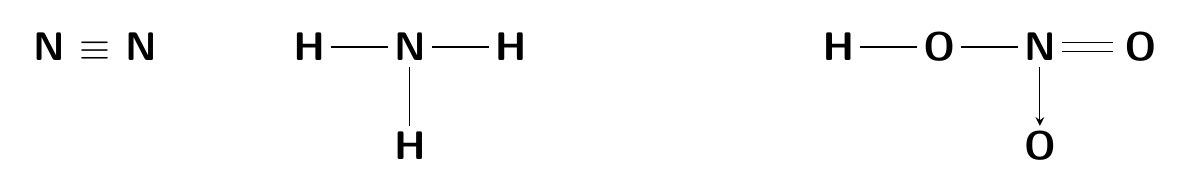
\begin{tikzpicture}[declare function={r=4;},font=\Large\sffamily\bfseries,inner sep=2pt]
			\path (r,0) node {N $\equiv$ N};
			%%%
			\path (2*r,0) node (nitrogen) {N};
			\draw (nitrogen)--++(-90:1cm) node [anchor=north] {H};
			\draw (nitrogen)--++(0:1cm) node [anchor=west] {H};
			\draw (nitrogen)--++(180:1cm) node [anchor=east] {H};
			%%%
			\path (4*r,0) node (nitrogen) {N};
			\draw[->,>=stealth] (nitrogen)--++(-90:1cm) node [anchor=north] {O};
			\draw([yshift=1.5pt]nitrogen.east)--++(0:0.65cm) ;
			\path (nitrogen)--++(0:1cm) node [anchor=west]{O};
			\draw([yshift=-1.5pt]nitrogen.east)--++(0:0.65cm);
			\draw (nitrogen)--++(180:1cm) node [anchor=east] (oxigen) {O};
			\draw (oxigen)--++(180:1cm) node [anchor=east] {H};
		\end{tikzpicture}
	\end{center}
	Số oxi hóa của nguyên tử N trong các phân tử trên lần lượt là
	\choice
	{0 ; -3 ; -4.}
	{0 ; +3 ; +5.}
	{-3 ; -3 ; +4.}
	{\True 0 ; -3 ; +5.}
	\loigiai{
		$N_2$: Do hai nguyên tử N giống nhau nên số oxi hóa của N là 0.
		\\
		$NH_3$: 
		\\Số oxi hóa của H là +1.
		\\Trong phân tử, tổng số oxi hóa của các nguyên tử bằng 0.
		\\Gọi số oxi hóa của N là $x$, ta có: $x + 3 \times (+1) = 0 \longrightarrow x = -3$.
		\\
		$HNO_3$: 
		\\Số oxi hóa của H là +1, của O là -2.
		\\Trong phân tử, tổng số oxi hóa của các nguyên tử bằng 0.
		\\Gọi số oxi hóa của N là $x$, ta có: $+1 + x + 3 \times (-2) = 0 \longrightarrow x = +5$.
	}
\end{ex}

\Closesolutionfile{ans}
\Closesolutionfile{ansex}
%\bangdapan{Ans-C04B01_Dang01}

%%%%%%%%%%%%%%%Trắc nghiệm đúng sai%%%%%%%%%%%%%%%%%%%%%%%%
\phan{Bài tập trắc nghiệm Đúng Sai}
%%%=============SOẠN EXTF===============%%%
\Opensolutionfile{ansex}[Ans/LGTF-C04B01_Dang1]
\Opensolutionfile{ansbook}[Ansbook/AnsTF-C04B01_Dang1]
\Opensolutionfile{ans}[Ans/Tempt-C04B01_Dang1]
	%%%=============EX_1=============%%%
	\begin{ex}
		\choiceTF
		{\True Chất khử là chất nhường electron, chất oxi hóa là chất nhận electron}
		{Chất khử là chất có số oxi hóa giảm sau phản ứng, chất oxi hóa là chất có số oxi hóa tăng sau phản ứng}
		{Chất khử tham gia vào quá trình khử, chất oxi hóa tham gia vào quá trình oxi hóa}
		{\True Chất khử và chất oxi hóa có thể là cùng một chất}
		\loigiai{}
	\end{ex}
	%%%=============EX_2=============%%%
	\begin{ex}
		\choiceTF
		{Quá trình khử là quá trình nhường e của chất khử}
		{\True Quá trình  oxi hóa là quá trình làm tăng số oxi hóa của một nguyên tố}
		{Quá trình oxi hóa là quá trình nhận e của chất oxi hóa}
		{\True Quá trình khử xảy ra đối với chất oxi hóa và quá trình oxi hóa xảy ra đối với chất khử}
		\loigiai{}
	\end{ex}
	%%%=============EX_3=============%%%
	\begin{ex}Xét vai trò của Clo trong phản ứng $Cl_2$ \explus $KOH$  $\xrightarrow$  $KCl$ \explus $KClO$ \explus $H_2O$
		\choiceTF
		{ $Cl_2 $ là chất oxi hóa $KOH$ là chất khử}
		{\True $Cl_2$ vừa là chất oxi hóa, vừa là chất khử}
		{$Cl_2 $tham gia vào quá trình khử và $KOH$ tham gia vào quá trình oxi hóa}
		{\True $ Cl_2 + 2e$  $\xrightarrow$ $2Cl^{-}$}
		\loigiai{}
	\end{ex}
	%%%=============EX_4=============%%%
	\begin{ex}
		Cho các phát biểu sau:
		\choiceTF
		{Trong tất cả các hợp chất số oxi hóa của H là +1}
		{\True Trong đơn chất, số oxi hoá của nguyên tử bằng 0}
		{\True Số oxi hóa là điện tích hình thức nếu giả định liên kết giứa các nguyên tử là liên kết ion}
		{\True Số oxi hóa của Alumium trong hợp chất $AlCl_3$ là +3}
		\loigiai{}
	\end{ex}
	%%%=============EX_5=============%%%
	\begin{ex}
		Cho các phát biểu sau:
		\choiceTF
		{Phản ứng oxi hóa là phản ứng có sự nhường và nhận proton}
		{\True Cho quá trình $Cu$  $\xrightarrow$  $Cu^{+2} +2e$, quá trình này gọi là quá trình oxi hóa}
		{\True Trong phản ứng oxi hóa - khử tổng số electron cho phải bằng tổng số electron nhận}
		{Phản ứng $CaCO_3$  $\xrightarrow[$t^\circ$]$ $CaO + CO_2$}
		\loigiai{}
	\end{ex}
	%%%=============EX_6=============%%%
	\begin{ex}
		Cho các phát biểu sau:
		\choiceTF
		{Chất oxi hoá là chất cho điện tử, chứa nguyên tố có số oxi hóa tăng sau phản ứng}
		{Chất khử là chất nhận điện tử, chứa nguyên tố có số oxi hóa tăng sau phản ứng}
		{Trong phân tử $NH_4NO_3$ thì số oxi hóa của 2 nguyên tử nitơ là: –3 và+5}
		{\True Cho quá trình: $Fe^{2+} \xrightarrow Fe^{3+}+1e$. Đây là quá trình oxi hóa}
		\loigiai{}
	\end{ex}
	%%%=============EX_7=============%%%
	\begin{ex}
		\choiceTF
		{Phản ứng $CaCO_3$  $\xrightarrow[$t^\circ$][xt]$  $CaO$  \explus  $CO_2$ là phản ứng oxi hóa - khử}
		{Chất oxi hóa tham gia vào quá trình oxi hóa}
		{Số oxi hóa của Al luôn là $+3$ trong tất cả các hợp chất}
		{\True Tỉ lệ số phân tử $HNO_3$ bị khử và tham gia gia môi trường tạo muối trong phản ứng:\\
			$Cu + HNO_3 $  $\xrightarrow$  $ Cu{(NO_3)}_2 + NO + H_2O$ là 3:1}
		\loigiai{}
	\end{ex}
	%%%=============EX_8=============%%%
	\begin{ex}
		Trong các phát biểu sau phát biểu nào đúng, phát biểu nào sai?
		\choiceTF
		{\True Phản ứng oxi hoá-khử là phản ứng luôn xảy ra đồng thời sự oxi hoá và sự khử}
		{Phản ứng oxi hoá-khử là phản ứng trong đó có sự thay đổi số oxi hoá của tất cả các nguyên tố hóa học}
		{\True Phản ứng oxi hoá-khử là phản ứng trong đó xảy ra sự trao đổi electron giữa các chất}
		{Phản ứng oxi hóa khử là phản ứng phải có ít nhất 2 chất tham gia trong đó có một chất là chất oxi hóa, một chất là chất khử}
		\loigiai{}
	\end{ex}
	%%%=============EX_9=============%%%
	\begin{ex}%[0H4Y1-1]
		Cho các phát biểu sau. Phát biểu nào sai?
		\choiceTF
		{Số oxi hóa không phải là điện tích thực của nguyên tử}
		{\True Phản ứng oxi hóa khử luôn xảy ra quá trình oxi hóa và quá trình khử}
		{\True Trong quá trình khử, chất oxi hóa bị khử về số oxi hóa thấp hơn}
		{Chất oxi hóa và chất khử phải là hai chất khác nhau}
		\loigiai{
			\begin{itemchoice}[T1,T2,T3,F4]
				\itemch Số oxi hóa là điện tích giả định khi coi liên kết giữa các nguyên tử là lien kết ion
				\itemch Phản ứng oxi hóa khử luôn xảy ra đồng thời quá trình oxi hóa và quá trình khử
				\itemch Trong quá trình khử, chất oxi hóa nhận thêm electron nên số oxi hóa giảm
				\itemch Chất oxi hóa và chất khử có thể là cùng một chất, một chất có thể vừa nhường electron và vừa nhận electron
			\end{itemchoice}
		}
	\end{ex}
	%%%=============EX_10=============%%%
	\begin{ex}
		Cho phản ứng sau:
		$aFe_2O_3+bCO \xrightarrow cFe+dCO_2$  (1)
		\choiceTF
		{\True Trong phản ứng (1) $Fe_2O_3$ là chất oxi hóa, CO là chất khử}
		{Trong phản ứng (1) 1 nguyên tử Fe trong $Fe_2O_3$ bị oxi hóa từ $+3$ xuống $0$}
		{Trong phản ứng (1) xảy ra quá trình khử: $C^{+2}+2e \longrightarrow C^{+4}$}
		{Phản ứng (1) có tổng các hệ số là $a+b+c+d=9$}
		\loigiai{
			\begin{itemchoice}[T1,F2,F3,T4]
				\itemch $Fe_2O_3$ là chất oxi hóa, CO là chất khử vì Fe trong $Fe_2O_3$ giảm số oxi hóa, C trong CO tăng số oxi hóa
				\itemch 1 nguyên tử Fe trong $Fe_2O_3$ bị khử từ $+3$ xuống $0$
				\itemch Trong phản ứng (1) xảy ra quá trình oxi hóa: $C^{+2}  \longrightarrow C^{+4}+2e$
				\itemch Phản ứng (1) có tổng các hệ số a, b, c,d nguyên tối giản bằng $=9$
			\end{itemchoice}
		}
	\end{ex}
	%%%=============EX_11=============%%%
	\begin{ex}
		Cho phản ứng sau:
		$aFeS_2 + bO_2 \xrightarrow[$t^\circ$] cFe_2O_3 + dSO_2$ (1) (với a, b, c, d là các số nguyên tối giản).
		\choiceTF
		{\True Trong phản ứng (1) $O_2$ là chất oxi hóa, $FeS_2$ là chất khử}
		{\True Trong phản ứng (1) $Fe$ bị oxi hóa từ $+2$ lên $+3$}
		{\True Trong phản ứng (1) xảy ra quá trình oxi hóa: $S^{-1} \xrightarrow S^{+4}+5e$}
		{Phản ứng (1) có tổng các hệ số là $a+b+c+d=25$}
		\loigiai{%
			\begin{itemchoice}[T1,F2,F3,T4]
				\itemch $O_2$ là chất oxi hóa, $FeS_2$ là chất khử vì O trong $O_2$ giảm số oxi hóa, Fe và S trong $FeS_2$ tăng số oxi hóa
				\itemch Fe trong $FeS_2$ bị oxi hóa từ $+2$ lên $+3$
				\itemch Trong phản ứng (1) xảy ra quá trình oxi hóa: $S^{-1} \xrightarrow S^{+4}+5e$
				\itemch Phản ứng (1) có tổng các hệ số là $4+11+2+8=25$
			\end{itemchoice}
		}
	\end{ex}
\Closesolutionfile{ans}
\Closesolutionfile{ansbook}
\Closesolutionfile{ansex}
%\bangdapanTF{AnsTF-C04B01_Dang1}

\begin{dang}{Bài tập định luật bảo toàn electron}\end{dang}
\begin{pp}
	\Noibat[\maunhan][][\faStar][]{Cơ sở lý thuyết}
	\\
	\indam[\maunhan]{Định Luật Bảo Toàn Electron:} Trong các phản ứng oxi hóa - khử, tổng số mol electron mà các chất khử cho đi bằng tổng số mol electron mà các chất oxi hóa nhận vào.
	\Noibat[\maunhan][][\faStar][]{Các Bước Giải:}
	\begin{cacbuoc}
		\item Viết các trình khử và quá trình oxi hóa
		\item Đặt ẩn là số mol các chất  liên quan đến yêu cầu bài toán
		\item Dựa vào quá trình khử và quá trình oxi hóa biểu diễn mol e nhường và mol e nhận theo mol chất
	\end{cacbuoc}
	\begin{center}
		\boxct[\maunhan][3pt][\sffamily]{mol e nhường (nhận) = mol chất $\times$ số e trao đổi}
	\end{center}
\end{pp}
%%%=============SOẠN BT===============%%%
\Opensolutionfile{ansbth}[Ans/LGBT-C04B01_Dang_02]
\Opensolutionfile{ansbt}[Ans/AnsBT-C04B01_Dang_02]
	%%%=============BT_01=============%%%
	\begin{bt}
		Cân bằng các phản ứng oxi hóa khử sau bằng phương pháp thăng bằng electron:
		\begin{enumerate}[a)]
			\item $KMnO_4 + H_2S \rightarrow MnSO_4 + S + K_2SO_4 + H_2O$
			\item $FeS_2 + HNO_3 \rightarrow Fe(NO_3)_3 + H_2SO_4 + NO_2 + H_2O$
		\end{enumerate}
		\loigiai{
			\begin{enumerate}[a)]
				\item $2KMnO_4 + 5H_2S + 3H_2SO_4 \rightarrow 2MnSO_4 + 5S + K_2SO_4 + 8H_2O$
				\item $FeS_2 + 18HNO_3 \rightarrow Fe(NO_3)_3 + 2H_2SO_4 + 15NO_2 + 7H_2O$
			\end{enumerate}
		}
	\end{bt}
	
	%%%=============BT_02=============%%%
	\begin{bt}
		Cho 11.2 gam Fe tác dụng với dung dịch $HNO_3$ loãng dư, thu được V lít khí NO (đktc) là sản phẩm khử duy nhất.
		\begin{enumerate}[a)]
			\item Viết phương trình phản ứng.
			\item Tính giá trị của V.
		\end{enumerate}
		\loigiai{
			\begin{enumerate}[a)]
				\item $3Fe + 8HNO_3 \rightarrow 3Fe(NO_3)_2 + 2NO + 4H_2O$
				\item Số mol Fe = $\dfrac{11{,}2}{56} = 0{,}2$ mol
				\\
				Theo phương trình, số mol NO = $\dfrac{2}{3}$ số mol Fe = $\dfrac{2}{3} \times 0{,}2 = \dfrac{2}{15}$ mol
				\\
				Thể tích NO = $\dfrac{2}{15} \times 22{,}4 = 2{,}987$ lít
			\end{enumerate}
		}
	\end{bt}
	%%%=============BT_03=============%%%
	\begin{bt}
		Hòa tan hoàn toàn 12 gam hỗn hợp X gồm Fe và Cu vào dung dịch $HNO_3$ đặc nóng dư, thu được 6,72 lít khí $NO_2$ (đktc) là sản phẩm khử duy nhất.
		\begin{enumerate}[a)]
			\item Viết phương trình phản ứng.
			\item Tính phần trăm khối lượng mỗi kim loại trong hỗn hợp X.
		\end{enumerate}
		\loigiai{
			\begin{enumerate}[a)]
				\item $Fe + 6HNO_3 \rightarrow Fe(NO_3)_3 + 3NO_2 + 3H_2O$
				\\
				$Cu + 4HNO_3 \rightarrow Cu(NO_3)_2 + 2NO_2 + 2H_2O$
				\item Số mol $NO_2$ = $\dfrac{6{,}72}{22{,}4} = 0{,}3$ mol
				\\
				Gọi số mol Fe và Cu lần lượt là x và y
				\\
				Ta có hệ phương trình:
				\\
				$56x + 64y = 12$
				\\
				$3x + 2y = 0{,}3$
				\\
				Giải hệ phương trình ta được x = 0,1; y = 0
				\\
				%Fe = $\dfrac{0{,}1 \times 56}{12} \times 100 = 46{,}67\%$
				\\
				%Cu = $100 - 46{,}67 = 53{,}33\%$
			\end{enumerate}
		}
	\end{bt}
	%%%=============BT_04=============%%%
	\begin{bt}
		Cho 10 gam hỗn hợp X gồm Mg và Al tác dụng với dung dịch $H_2SO_4$ đặc nóng dư, thu được 11,2 lít khí $SO_2$ (đktc) là sản phẩm khử duy nhất.
		\begin{enumerate}[a)]
			\item Viết phương trình phản ứng.
			\item Tính phần trăm khối lượng mỗi kim loại trong hỗn hợp X.
		\end{enumerate}
		\loigiai{
			\begin{enumerate}[a)]
				\item $Mg + 2H_2SO_4 \rightarrow MgSO_4 + SO_2 + 2H_2O$
				\\
				$2Al + 6H_2SO_4 \rightarrow Al_2(SO_4)_3 + 3SO_2 + 6H_2O$
				\item Số mol $SO_2$ = $\dfrac{11{,}2}{22{,}4} = 0{,}5$ mol
				\\
				Gọi số mol Mg và Al lần lượt là x và y
				\\
				Ta có hệ phương trình:
				\\
				$24x + 27y = 10$
				\\
				$x + 1{,}5y = 0{,}5$
				\\
				Giải hệ phương trình ta được $x = 0{,}2; y = 0{,}2$
				\\
				\% Mg = $\dfrac{0{,}2 \times 24}{10} \times 100 = 48 \%$
				\\
				\% Al = $100 - 48 = 52\%$
			\end{enumerate}
		}
	\end{bt}
	%%%=============BT_05=============%%%
	\begin{bt}
		Cho 20 gam hỗn hợp X gồm Fe và FeO tác dụng với dung dịch $HNO_3$ loãng dư, thu được 5,6 lít khí NO (đktc) là sản phẩm khử duy nhất.
		\begin{enumerate}[a)]
			\item Viết phương trình phản ứng.
			\item Tính phần trăm khối lượng mỗi chất trong hỗn hợp X.
		\end{enumerate}
		\loigiai{
			\begin{enumerate}[a)]
				\item $3Fe + 8HNO_3 \rightarrow 3Fe(NO_3)_2 + 2NO + 4H_2O$
				\\
				$3FeO + 10HNO_3 \rightarrow 3Fe(NO_3)_3 + NO + 5H_2O$
				\item Số mol NO = $\dfrac{5{,}6}{22{,}4} = 0{,}25$ mol
				\\
				Gọi số mol Fe và FeO lần lượt là x và y
				\\
				Ta có hệ phương trình:
				\\
				$56x + 72y = 20$
				\\
				$\dfrac{2}{3}x + \dfrac{1}{3}y = 0{,}25$
				\\
				Giải hệ phương trình ta được $x = 0{,}15; y = 0{,}1$
				\\
				$\%Fe$ = $\dfrac{0{,}15 \times 56}{20} \times 100 = 42\%$
				\\
				$\%FeO$ = $100 - 42 = 58\%$
			\end{enumerate}
		}
	\end{bt}
	%%%=============BT_6=============%%%
	\begin{bt}
		Hàm lượng iron(II) sulfate được xác định qua phản ứng oxi hoá - khử với potassium permanganate:
		\begin{equation*}
			\text{FeSO}_4 + \text{KMnO}_4 + \text{H}_2\text{SO}_4 \rightarrow \text{Fe}_2(\text{SO}_4)_3 + \text{K}_2\text{SO}_4 + \text{MnSO}_4 + \text{H}_2\text{O}
		\end{equation*}
		\begin{enumerate}[a)]
			\item Lập phương trình hoá học của phản ứng theo phương pháp thăng bằng electron. Chỉ rõ chất oxi hoá, chất khử.
			\item Tính thể tích dung dịch \text{KMnO}\textsubscript{4} 0,02 M để phản ứng vừa đủ với 20 mL dung dịch \text{FeSO}\textsubscript{4} 0,10 M.
		\end{enumerate}
		\loigiai{
			\begin{enumerate}[a)]
				\item Quá trình oxi hóa:
				\[2\times \left( \overset{+2}{\text{Fe}} \rightarrow \overset{+3}{\text{Fe}} + 1e \right)\]
				Quá trình khử:
				\[1\times \left( \overset{+7}{\text{Mn}} + 5e \rightarrow \overset{+2}{\text{Mn}} \right)\]
				Phương trình hóa học:
				\[10\text{FeSO}_4 + 2\text{KMnO}_4 + 8\text{H}_2\text{SO}_4 \rightarrow 5\text{Fe}_2(\text{SO}_4)_3 + \text{K}_2\text{SO}_4 + 2\text{MnSO}_4 + 8\text{H}_2\text{O}\]
				Chất oxi hóa: $\text{KMnO}_4$, chất khử: $\text{FeSO}_4$.
				\item Số mol $\text{FeSO}_4$ là:
				\[n_{\text{FeSO}_4} = 0{,}10 \times 0{,}02 = 0{,}002 \text{ mol}\]
				Theo phương trình phản ứng, ta có:
				\[n_{\text{KMnO}_4} = \frac{1}{5} n_{\text{FeSO}_4} = \frac{1}{5} \times 0{,}002 = 0{,}0004 \text{ mol}\]
				Thể tích dung dịch $\text{KMnO}_4$ cần dùng là:
				\[V_{\text{KMnO}_4} = \frac{0{,}0004}{0{,}02} = 0{,}02 \text{ lít} = 20 \text{ mL}\]
			\end{enumerate}
		}
	\end{bt}
	%%%=============BT_7=============%%%
	\begin{bt}
		Cho $2{,}34$ g kim loại M (hoá trị n) tác dụng với dung dịch \text{H}\textsubscript{2}\text{SO}\textsubscript{4} (đặc, nóng, dư) thu được $3{,}2227$ L khí \text{SO}\textsubscript{2} (điều kiện chuẩn). Xác định kim loại M.
		\loigiai{
			Số mol khí \text{SO}\textsubscript{2} thu được là:
			\[n_{\text{SO}_2} = \frac{3{,}2227}{22{,}4} = 0{,}144 \text{ mol}\]
			Phương trình phản ứng tổng quát:
			\[2M + 2n\text{H}_2\text{SO}_4 \rightarrow M_2(\text{SO}_4)_n + n\text{SO}_2 + 2n\text{H}_2\text{O}\]
			Theo phương trình, số mol kim loại M là:
			\[n_M = \frac{2}{n} n_{\text{SO}_2} = \frac{2}{n} \times 0{,}144 = \frac{0{,}288}{n}\]
			Khối lượng mol của kim loại M là:
			\[M_M = \frac{2{,}34}{\frac{0{,}288}{n}} = \frac{2{,}34n}{0{,}288} = 8{,}125n\]
			Xét các trường hợp n = 1, 2, 3:
			\begin{itemize}
				\item Nếu n = 1, $M_M = 8{,}125$ (loại)
				\item Nếu n = 2, $M_M = 16{,}25$ (loại)
				\item Nếu n = 3, $M_M = 24{,}375$ (Al)
			\end{itemize}
			Vậy kim loại M là Al (Nhôm).
		}
	\end{bt}
	%%%=============BT_8=============%%%
	\begin{bt}
		Cho 11,2 gam Fe tác dụng với dung dịch HNO3 loãng dư thu được V lít khí NO (đktc) và dung dịch X.
		\begin{enumerate}[a)]
			\item Viết phương trình phản ứng xảy ra.
			\item Tính giá trị của V.
			\item Cô cạn dung dịch X thu được bao nhiêu gam muối khan?
		\end{enumerate}
		\loigiai{
			\begin{enumerate}[a)]
				\item Phương trình phản ứng:
				\[3Fe + 8HNO_3 \rightarrow 3Fe(NO_3)_2 + 2NO + 4H_2O\]
				\item Số mol Fe:
				\[n_{Fe} = \frac{11{,}2}{56} = 0{,}2 \text{ mol}\]
				Theo phương trình phản ứng, số mol NO:
				\[n_{NO} = \frac{2}{3} n_{Fe} = \frac{2}{3} \times 0{,}2 = \frac{0{,}4}{3} \text{ mol}\]
				Thể tích khí NO:
				\[V_{NO} = \frac{0{,}4}{3} \times 22{,}4 = 2{,}987 \text{ lít}\]
				\item Số mol $Fe(NO_3)_2$:
				\[n_{Fe(NO_3)_2} = n_{Fe} = 0{,}2 \text{ mol}\]
				Khối lượng muối khan:
				\[m_{Fe(NO_3)_2} = 0{,}2 \times 180 = 36 \text{ gam}\]
			\end{enumerate}
		}
	\end{bt}
	%%%=============BT_9=============%%%
	\begin{bt}
		Cho m gam hỗn hợp X gồm Fe và Cu tác dụng với dung dịch $H_2SO_4$ đặc nóng dư, thu được dung dịch Y và khí $SO_2$. Cho dung dịch Y tác dụng với dung dịch NaOH dư, thu được kết tủa Z. Nung Z trong không khí đến khối lượng không đổi, thu được 16 gam chất rắn. Mặt khác, cho m gam hỗn hợp X tác dụng với dung dịch HCl dư, thu được $2{,}24$ lít khí $H_2$ (đktc). Tính giá trị của m.
		\loigiai{
			Khi cho X tác dụng với HCl, chỉ Fe phản ứng:
			\[Fe + 2HCl \rightarrow FeCl_2 + H_2\]
			Số mol H2:
			\[n_{H_2} = \frac{2{,}24}{22{,}4} = 0{,}1 \text{ mol}\]
			Số mol Fe:
			\[n_{Fe} = n_{H_2} = 0{,}1 \text{ mol}\]
			Khi cho X tác dụng với H2SO4 đặc nóng:
			\[2Fe + 6H_2SO_4 \rightarrow Fe_2(SO_4)_3 + 3SO_2 + 6H_2O\]
			\[Cu + 2H_2SO_4 \rightarrow CuSO_4 + SO_2 + 2H_2O\]
			Dung dịch Y chứa $Fe_2(SO_4)_3$ và $CuSO_4$.
			Khi cho Y tác dụng với NaOH:
			\[Fe_2(SO_4)_3 + 6NaOH \rightarrow 2Fe(OH)_3 + 3Na_2SO_4\]
			\[CuSO_4 + 2NaOH \rightarrow Cu(OH)_2 + Na_2SO_4\]
			Kết tủa Z gồm $Fe(OH)_3$ và $Cu(OH)_2$.
			Nung Z trong không khí:
			\[2Fe(OH)_3 \rightarrow Fe_2O_3 + 3H_2O\]
			\[Cu(OH)_2 \rightarrow CuO + H_2O\]
			Chất rắn thu được là $Fe_2O_3$ và $CuO$.
			Số mol $Fe_2O_3$:
			\[n_{Fe_2O_3} = \frac{1}{2} n_{Fe} = \frac{1}{2} \times 0{,}1 = 0{,}05 \text{ mol}\]
			Khối lượng $Fe_2O_3$:
			\[m_{Fe_2O_3} = 0{,}05 \times 160 = 8 \text{ gam}\]
			Khối lượng CuO:
			\[m_{CuO} = 16 - 8 = 8 \text{ gam}\]
			Số mol CuO:
			\[n_{CuO} = \frac{8}{80} = 0{,}1 \text{ mol}\]
			Số mol Cu:
			\[n_{Cu} = n_{CuO} = 0{,}1 \text{ mol}\]
			Khối lượng hỗn hợp X:
			\[m = m_{Fe} + m_{Cu} = 0{,}1 \times 56 + 0{,}1 \times 64 = 12 \text{ gam}\]
		}
	\end{bt}
	%%%=============BT_10=============%%%
	\begin{bt}
		Hòa tan hoàn toàn 10 gam hỗn hợp X gồm Fe và FeO bằng dung dịch HCl dư, thu được $2{,}24$ lít khí $H_2$ (đktc) và dung dịch Y. Cô cạn dung dịch Y thu được m gam muối khan. Tính giá trị của m.
		\loigiai{
			Số mol $H_2$:
			\[n_{H_2} = \frac{2{,}24}{22{,}4} = 0{,}1 \text{ mol}\]
			Chỉ Fe phản ứng với HCl tạo $H_2$:
			\[Fe + 2HCl \rightarrow FeCl_2 + H_2\]
			Số mol Fe:
			\[n_{Fe} = n_{H_2} = 0{,}1 \text{ mol}\]
			Khối lượng Fe:
			\[m_{Fe} = 0{,}1 \times 56 = 5{,}6 \text{ gam}\]
			Khối lượng FeO:
			\[m_{FeO} = 10 - 5{,}6 = 4{,}4 \text{ gam}\]
			Số mol FeO:
			\[n_{FeO} = \frac{4{,}4}{72} = \frac{11}{180} \text{ mol}\]
			FeO tác dụng với HCl:
			\[FeO + 2HCl \rightarrow FeCl_2 + H_2O\]
			Số mol $FeCl_2$ từ FeO:
			\[n_{FeCl_2 (FeO)} = n_{FeO} = \frac{11}{180} \text{ mol}\]
			Số mol $FeCl_2$ từ Fe:
			\[n_{FeCl_2 (Fe)} = n_{Fe} = 0{,}1 \text{ mol}\]
			Tổng số mol $FeCl_2$:
			\[n_{FeCl_2} = \frac{11}{180} + 0{,}1 = \frac{29}{180} \text{ mol}\]
			Khối lượng muối khan:
			\[m_{FeCl_2} = \frac{29}{180} \times 127 = 20{,}46 \text{ gam}\]
		}
	\end{bt}
\Closesolutionfile{ansbt}
\Closesolutionfile{ansbth}
%\bangdapanSA{AnsBT-C04B01_Dang_02}
